%%%%%%%%%%%%%%%%%%%%%%%%%%%%%%%%%%%%%%%%%%%%%%%%%%%%%%%%%%%%%%%%%%%%%%%%%%%%%%%%
%% Plantilla de memoria en LaTeX para la EIF - Universidad Rey Juan Carlos
%%
%% Por Gregorio Robles <grex arroba gsyc.urjc.es>
%%     Grupo de Sistemas y Comunicaciones
%%     Escuela de Ingeniería de Fuenlabrada
%%     Universidad Rey Juan Carlos
%% (muchas ideas tomadas de Internet, colegas del GSyC, antiguos alumnos...
%%  etc. Muchas gracias a todos)
%%
%% La última versión de esta plantilla está siempre disponible en:
%%     https://github.com/gregoriorobles/plantilla-memoria
%%
%% Para obtener PDF, ejecuta en la shell:
%%   make
%% (las imágenes deben ir en PNG o JPG)

%%%%%%%%%%%%%%%%%%%%%%%%%%%%%%%%%%%%%%%%%%%%%%%%%%%%%%%%%%%%%%%%%%%%%%%%%%%%%%%%

\documentclass[a4paper, 12pt]{book}
%\usepackage[T1]{fontenc}

\usepackage[a4paper, left=2.5cm, right=2.5cm, top=3cm, bottom=3cm]{geometry}
\usepackage{times}
\usepackage[utf8]{inputenc}
\usepackage[spanish]{babel} % Comenta esta línea si tu memoria es en inglés
\usepackage{url}
\usepackage{color}
%\usepackage[dvipdfm]{graphicx}
\usepackage{graphicx}
\usepackage{subfigure}
\usepackage{float}  %% H para posicionar figuras
\usepackage[nottoc, notlot, notlof, notindex]{tocbibind} %% Opciones de índice
\usepackage{latexsym}  %% Logo LaTeX
\usepackage{listings}
\usepackage{xcolor}
\usepackage{tikz}
\usepackage{amsmath}
\usepackage{subcaption}
\usepackage{subfig}

\usetikzlibrary{shapes.geometric, arrows}


\tikzstyle{startstop} = [rectangle, rounded corners, minimum width=2cm, minimum height=0.6cm, text centered, draw=black, fill=red!30]
\tikzstyle{process} = [rectangle, minimum width=2cm, minimum height=0.6cm, text centered, draw=black, fill=orange!30]
\tikzstyle{decision} = [diamond, minimum width=2cm, minimum height=0.6cm, text centered, draw=black, fill=green!30]
\tikzstyle{arrow} = [thick,->,>=stealth]

\title{Memoria del Proyecto}
\author{Nombre del autor}

\renewcommand{\baselinestretch}{1.5}  %% Interlineado

\lstset{ 
	language=Python, 
	basicstyle=\ttfamily\small, 
	keywordstyle=\color{blue}\bfseries, 
	commentstyle=\color{green}, 
	stringstyle=\color{red}, 
	showstringspaces=false,
	numbers=left,
	numberstyle=\tiny\color{gray},
	stepnumber=1,
	numbersep=5pt,
	tabsize=4,
	breaklines=true,
	breakatwhitespace=false,
	frame=single,
	captionpos=b
}


\begin{document}
	
	\renewcommand{\refname}{Bibliografía}  %% Renombrando
	\renewcommand{\appendixname}{Apéndice}
	
	
	%%%%%%%%%%%%%%%%%%%%%%%%%%%%%%%%%%%%%%%%%%%%%%%%%%%%%%%%%%%%%%%%%%%%%%%%%%%%%%%%
	% PORTADA
	
	\begin{titlepage}
		\begin{center}
			\includegraphics[scale=0.6]{img/URJ_logo_Color_POS.png}
			
			\vspace{1.75cm}
			
			\LARGE
			ESCUELA DE INGENIERÍA DE FUENLABRADA
			\vspace{1cm}
			
			\LARGE
			GRADO EN INGENIERÍA EN TECNOLOGÍAS DE LA TELECOMUNICACIÓN
			
			\vspace{1cm}
			\LARGE
			\textbf{TRABAJO FIN DE GRADO}
			
			\vspace{1cm}
			
			\Large
			CONFIGURACIÓN Y MEDIDAS DE UN PLANO DE CONTROL IN-BAND SDN EN EL ENTORNO DE EMULACIÓN DE REDES MININET
			
			\vspace{2cm}
			
			\large
			Autor : Luis Haro Peña \\
			Tutor : Pedro de las Heras Quirós\\
			Contutora: Eva María Castro Barbero
			\vspace{1cm}
			
			\large
			Curso académico 2023/2024
			
		\end{center}
	\end{titlepage}
	
	\newpage
	\mbox{}
	\thispagestyle{empty} % para que no se numere esta pagina
	
	
	
	%%%%%%%%%%%%%%%%%%%%%%%%%%%%%%%%%%%%%%%%%%%%%%%%%%%%%%%%%%%%%%%%%%%%%%%%%%%%%%%%
	%%%% Para firmar
	\clearpage
	\pagenumbering{gobble}
	\chapter*{}
	
	\vspace{-4cm}
	\begin{center}
		\LARGE
		\textbf{Trabajo Fin de Grado}
		
		\vspace{1cm}
		\large
		Configuración y medidas de un plano de control In-Band SDN en el entorno de emulación de redes Mininet.
		
		\vspace{1cm}
		\large
		\textbf{Autor :} Luis Haro Peña \\
		\textbf{Tutor :} Pedro de las Heras Quirós \\
		\textbf{Contutora :} Eva María Castro Barbero
		
	\end{center}
	
	\vspace{1cm}
	La defensa del presente Trabajo fin de grado se realizó el día \qquad$\;\,$ de \qquad\qquad\qquad\qquad \newline de 2024, siendo calificada por el siguiente tribunal:
	
	
	\vspace{0.5cm}
	\textbf{Presidente:}
	
	\vspace{1.2cm}
	\textbf{Secretario:}
	
	\vspace{1.2cm}
	\textbf{Vocal:}
	
	
	\vspace{1.2cm}
	y habiendo obtenido la siguiente calificación:
	
	\vspace{1cm}
	\textbf{Calificación:}
	
	
	\vspace{1cm}
	\begin{flushright}
		Fuenlabrada, a \qquad$\;\,$ de \qquad\qquad\qquad\qquad de 2024
	\end{flushright}
	

	%%%%%%%%%%%%%%%%%%%%%%%%%%%%%%%%%%%%%%%%%%%%%%%%%%%%%%%%%%%%%%%%%%%%%%%%%%%%%%%%
	%%%% Resumen
	
	\chapter*{Resumen}
	%\addcontentsline{toc}{chapter}{Resumen} % si queremos que aparezca en el índice
	\markboth{RESUMEN}{RESUMEN} % encabezado
	Este trabajo de fin de grado se centra en la configuración y realización de medidas de parámetros 
	de un plano de control in-band basado en SDN/OpenFlow denominado Periplus. La
	creciente demanda de redes más flexibles, escalables y programables ha impulsado el desarrollo de 
	nuevas tecnologías como las Redes Definidas por Software (Software Defined Networks, SDN). 
	El protocolo estándar que se utiliza en este tipo de redes en la denominada interfaz sur es
	OpenFlow. 
	
	En este contexto, se busca estudiar el funcionamiento de Periplus, un plano de control  inband que utiliza 
	OpenFlow. Se analizará su rendimiento en diferentes escenarios de red para valorar su comportamiento 
	al arrancar varias topologías de redes, ejecutando una o varias instancias del controlador 
	en el entorno de emulación de redes Mininet.
	
	Mininet es un entorno que permite emular escenarios de red de forma sencilla a través de scripts de 
	Python que definen máquinas virtuales y la conexión de las mismas a través de Open vSwitch.
	
	Con el desarrollo de este trabajo fin de grado se han podido evaluar medidas de tiempo de conexión de todos los
	switches al controlador Periplus. Los resultados han mostrado que el factor determinante en este tiempo
	es la distancia en número de saltos desde el switch más lejano de la topología al controlador. En escenarios
	multicontrolador esta distancia disminuye y en general se obtienen mejoras en las medidas de tiempo
	de conexión de todos los switches. Otra característica que se ha analizado es el reparto de la gestión de los
	switches entre los difeferenes controladores. Los resultados han mostrado que este reparto suele ser equilibrado.
	
	%%%%%%%%%%%%%%%%%%%%%%%%%%%%%%%%%%%%%%%%%%%%%%%%%%%%%%%%%%%%%%%%%%%%%%%%%%%%%%%%
	%%%% Resumen en inglés
	
	\chapter*{Summary}
	%\addcontentsline{toc}{chapter}{Summary} % si queremos que aparezca en el índice
	\markboth{SUMMARY}{SUMMARY} % encabezado
	
This final degree work is focused on the configuration and parameter measurements of an SDN/Openflow based inband control plane called Periplus. The demand for more flexible, scalable and programmable networks has driven the development of new technologies such as Software Defined Networks (SDN). The standard protocol used in this type of network at the so-called southern interface is
OpenFlow. 

In this context, the aim is to study the performance of Periplus, an inband control plane using OpenFlow. Its performance will be analyzed in different network scenarios to assess its behavior when starting various network topologies, running one or several instances of the controller in the Mininet network emulation environment.

Mininet is an environment that allows to emulate network scenarios in a simple way through Python scripts that define virtual machines and connect them through Open vSwitch. Python scripts that define virtual machines and their connection through Open vSwitch.


With the development of this final degree work, it has been possible to evaluate the connection time measurements of all the switches to the Periplus controller. The results have shown that the determining factor in this time is the distance in number of hops from the farthest switch in the topology to the controller. In multicontroller scenarios this distance decreases and, in general, improvements are obtained in the connection time measurements of all the switches. 
Another feature that has been analyzed is the distribution of switch management among the different controllers. The results have shown that this distribution is usually balanced.


	%%%%%%%%%%%%%%%%%%%%%%%%%%%%%%%%%%%%%%%%%%%%%%%%%%%%%%%%%%%%%%%%%%%%%%%%%%%%%%%%
	%%%%%%%%%%%%%%%%%%%%%%%%%%%%%%%%%%%%%%%%%%%%%%%%%%%%%%%%%%%%%%%%%%%%%%%%%%%%%%%%
	% ÍNDICES %
	%%%%%%%%%%%%%%%%%%%%%%%%%%%%%%%%%%%%%%%%%%%%%%%%%%%%%%%%%%%%%%%%%%%%%%%%%%%%%%%%
	
	% Las buenas noticias es que los índices se generan automáticamente.
	% Lo único que tienes que hacer es elegir cuáles quieren que se generen,
	% y comentar/descomentar esa instrucción de LaTeX.
	
	%%%% Índice de contenidos
	\tableofcontents 
	%%%% Índice de figuras
	\cleardoublepage
	%\addcontentsline{toc}{chapter}{Lista de figuras} % para que aparezca en el indice de contenidos
	\listoffigures % indice de figuras
	%%%% Índice de tablas
	%\cleardoublepage
	%\addcontentsline{toc}{chapter}{Lista de tablas} % para que aparezca en el indice de contenidos
	%\listoftables % indice de tablas
	
	
	%%%%%%%%%%%%%%%%%%%%%%%%%%%%%%%%%%%%%%%%%%%%%%%%%%%%%%%%%%%%%%%%%%%%%%%%%%%%%%%%
	%%%%%%%%%%%%%%%%%%%%%%%%%%%%%%%%%%%%%%%%%%%%%%%%%%%%%%%%%%%%%%%%%%%%%%%%%%%%%%%%
	% INTRODUCCIÓN %
	%%%%%%%%%%%%%%%%%%%%%%%%%%%%%%%%%%%%%%%%%%%%%%%%%%%%%%%%%%%%%%%%%%%%%%%%%%%%%%%%
	
	\clearpage
	\chapter{Introducción}
	\label{sec:intro} % etiqueta para poder referenciar luego en el texto con ~\ref{sec:intro}
	\pagenumbering{arabic} % para empezar la numeración de página con números
	
	
	En el ámbito de las telecomunicaciones, la evolución constante de las redes y la creciente demanda de mayor flexibilidad y eficiencia han impulsado el surgimiento de nuevas tecnologías y enfoques de gestión de redes. Entre ellos, destaca la Red Definida por Software (SDN)[4] y el protocolo OpenFlow[2], los cuales han revolucionado la forma en que se configuran y controlan las redes. En este contexto, el presente trabajo de fin de grado se enfoca en la configuración y medidas de un plano de control in-band SDN/OpenFlow[1], específicamente en un entorno de emulación de redes: Mininet.
	
	El objetivo principal de este trabajo es explorar las capacidades y ventajas que ofrece la implementación de un plano de control in-band SDN/OpenFlow en una infraestructura de red basada en switches Ethernet. A través de la configuración y pruebas exhaustivas, se busca demostrar la viabilidad y el potencial de esta solución en términos de gestión centralizada, flexibilidad y escalabilidad. Además, se abordará el aspecto de la robustez, ya que la introducción de un plano de control centralizado también conlleva desafíos en cuanto a problemas en la red debido a que un enlace o un switch dejen de funcionar, provocando problemas de comunicación entre los dispositivos.
	
	
	En este capítulo se va a realizar una introducción a la temática de este trabajo de fin de grado. Por una
	parte se definirá qué son las redes definidas por software y el protocolo de comunicaciones que
	se utiliza mayoritariamente en estos entornos OpenFlow. A continuación se mostrará el entorno
	de trabajo y las herramientas necesarias para la realización de este trabajo fin de grado.
	
	
	\section{Redes de Ordenadores} 
	\label{sec:redes}
	
	Las redes de ordenadores son sistemas interconectados que permiten la comunicación y el intercambio de datos entre diferentes dispositivos informáticos. Estas redes pueden ser locales (LAN), que conectan dispositivos en un área geográfica limitada, o extenderse a través de distancias más grandes, como en las redes de área amplia (WAN) o incluso redes globales como Internet.
	
	En una red de ordenadores, los dispositivos, como computadoras, servidores, impresoras y dispositivos de almacenamiento, se conectan mediante cables o tecnologías inalámbricas. La comunicación se facilita a través de protocolos y estándares, como TCP/IP (Protocolo de Control de Transmisión/Protocolo de Internet).
	
	En las redes TCP/IP, los dispositivos de red tienen integradas funcionalidades de
	control y de reenvío de datos para la configuración	y el funcionamiento general de los dispositivos. 
	
	\section{Redes Definidas por Software} 
	\label{sec:sdn}
	
	Redes Definidas por Software (Software defined Networking, SDN), es una arquitectura de red que busca mejorar la flexibilidad y el control de las redes mediante la separación del plano de control y el plano de datos, véase la figura \ref{figura:SDN}. En las redes tradicionales, estos dos planos están integrados en los dispositivos de red, como switches y routers.
	
	En un entorno SDN, el plano de control se centraliza en una aplicación denominada controlador SDN, que es un software que tiene una visión global de la red y toma decisiones sobre cómo debe ser dirigido el tráfico. El plano de datos, que se ocupa de la transmisión real de los datos, permanece distribuido en los dispositivos de red. La comunicación entre el controlador y los dispositivos se realiza a través de protocolos estandarizados, como OpenFlow. El controlador configura los dispositivos de la red para que implementen el reenvío de datos en el plano de datos.
	
	Los beneficios de SDN incluyen una mayor flexibilidad y agilidad para adaptarse a cambios en la red, una gestión más centralizada que facilita la automatización y la programabilidad de la red, y una mayor eficiencia en la utilización de los recursos de red.
	
	
	\begin{figure}[H]
		\centering
		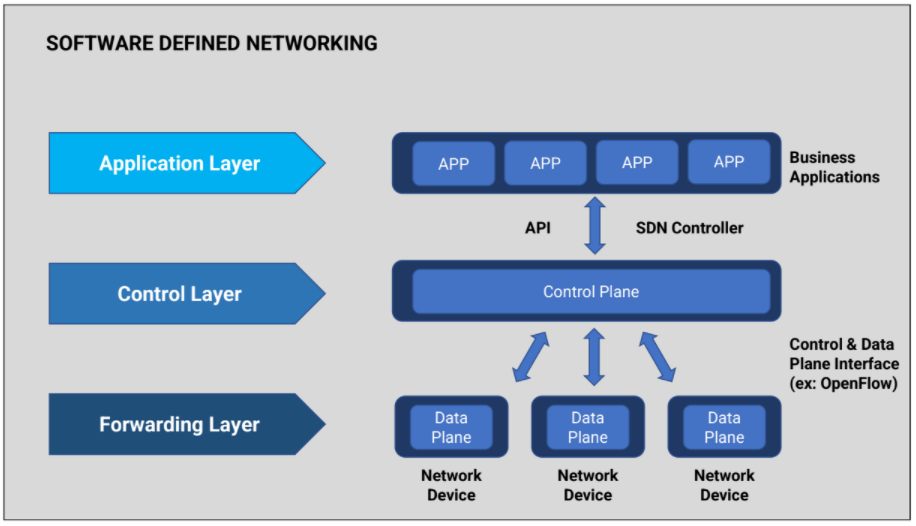
\includegraphics[width=14cm, keepaspectratio]{img/SDN}
		\caption{Plano de control y de datos en SDN.}
		\label{figura:SDN}
	\end{figure}
	
	\section{OpenFlow}
	\label{sec:openflow}
	
	
	OpenFlow [13] es un protocolo de comunicaciones que fue desarrollado por la Open Networking Foundation (ONF) y se ha convertido en un estándar abierto utilizado en redes definidas por software.
	Un controlador SDN toma decisiones sobre el funcionamiento de la red y configura los dispositivos de red para que los implementen. Para ello, el controlador debe enviar a los dispositivos de red mensajes que permitan configurar acciones para realizar la función de encaminamiento. Uno de los protocolos que se ha convertido en estándar para la comunicación entre el controlador y los dispositivos de red es OpenFlow. Los dispositivos de red compatibles con OpenFlow, reciben mensajes  OpenFlow del controlador y actúan como ejecutores de las intrucciones proporcionadas por dicho controlador.
	
	El protocolo OpenFlow establece una conexión TCP entre el controlador y los dispositivos de red  y define un conjunto de mensajes para la comunicación entre ellos. El controlador puede enviar instrucciones a los dispositivos de red, como reglas de flujo, y recibir información sobre el estado de la red de los dispositivos de red, como estadísticas de tráfico. Esto permite una gestión centralizada y programable de la red, lo que facilita que el controlador pueda llevar a cabo la implementación de políticas de red, la optimización del tráfico y la resolución de problemas.

	
	Algunas de las ventajas de OpenFlow y SDN incluyen la flexibilidad y la capacidad de adaptación de la red a las necesidades cambiantes, la simplificación de la administración y la configuración de la red, y la posibilidad de implementar nuevas funcionalidades y servicios de manera más rápida y eficiente.
	
	En el cuadro 1.1 podemos observar algunos de los mensajes más importantes de  OpenFlow y sus funciones.
	
	\begin{table}[H] % Fija la tabla en esta posición
		\centering
	
	
		\begin{tabular}{|c|l|}
			\hline
			\textbf{Mensaje} & \textbf{Función} \\
			\hline
			\texttt{OFPT\_HELLO} & Mensaje de saludo para iniciar la conexión \\
			\hline
			\texttt{OFPT\_FEATURES\_REQUEST} & Solicita información sobre las características del switch \\
			\hline
			\texttt{OFPT\_FEATURES\_REPLY} & Responde con información sobre las características del switch \\
			\hline
			\texttt{OFPT\_FLOW\_MOD} & Modifica el flujo de tráfico en el switch \\
			\hline
			\texttt{OFPT\_PACKET\_IN} & Indica la llegada de un paquete al switch \\
			\hline
			\texttt{OFPT\_PACKET\_OUT} & Envía un paquete fuera del switch \\
			\hline
			\texttt{OFPT\_FLOW\_REMOVED} & Indica que un flujo ha sido borrado del switch \\
			\hline
			\texttt{OFPT\_ERROR} & Indica un error en la comunicación \\
			\hline
			\texttt{OFPT\_ECHO\_REQUEST} & Solicita una respuesta de eco \\
			\hline
			\texttt{OFPT\_ECHO\_REPLY} & Responde a una solicitud de eco \\
			\hline
			\texttt{OFPT\_GET\_CONFIG\_REQUEST} & Solicita la configuración actual del switch \\
			\hline
			\texttt{OFPT\_SET\_CONFIG} & Establece la configuración del switch \\
			\hline
		\end{tabular}
		\label{tab:openflow}
		\caption{Mensajes OpenFlow y sus funciones}
	\end{table}
	
	\section{Open vSwitch} 
	\label{sec:vswitch}
	
	Open vSwitch (OVS) [6] es un switch virtual de código abierto diseñado para su uso en entornos de virtualización y redes definidas por software. Se integra con hipervisores como KVM (Kernel-based Virtual Machine), Xen, y es compatible con plataformas de virtualización como VMware.
	
	Algunas características clave de Open vSwitch incluyen:
	
	\begin{enumerate}
		\item Conmutación Virtual: Open vSwitch permite la conmutación de paquetes a nivel de hipervisor, facilitando la comunicación entre máquinas virtuales (VM) y con la red física.
		
		\item Soporte SDN: Se puede utilizar en entornos SDN, ya que es compatible con el protocolo OpenFlow. Esto permite una gestión centralizada y programable de la red.
		
		\item Compatibilidad Multiplataforma: Puede funcionar en una variedad de sistemas operativos, incluyendo Linux y Windows.
		
		\item Reenvío y Encaminamiento: Ofrece funcionalidades de reenvío a nivel de capa 2 y encaminamiento en capa 3, lo que significa que puede operar en diferentes capas de la arquitectura TCP/IP para proporcionar conectividad..
		
		\item Port Mirroring: Permite la replicación selectiva del tráfico de red para su análisis y monitorización.
		
	\end{enumerate}
	
	Open vSwitch es una herramienta versátil que se ha convertido en una opción popular en entornos de virtualización debido a su capacidad para integrarse con diversas tecnologías y sistemas de gestión de red. Su naturaleza de código abierto también facilita la adaptación y personalización, según las necesidades específicas de un entorno de red.
	
	\begin{figure}[H]
		\centering
		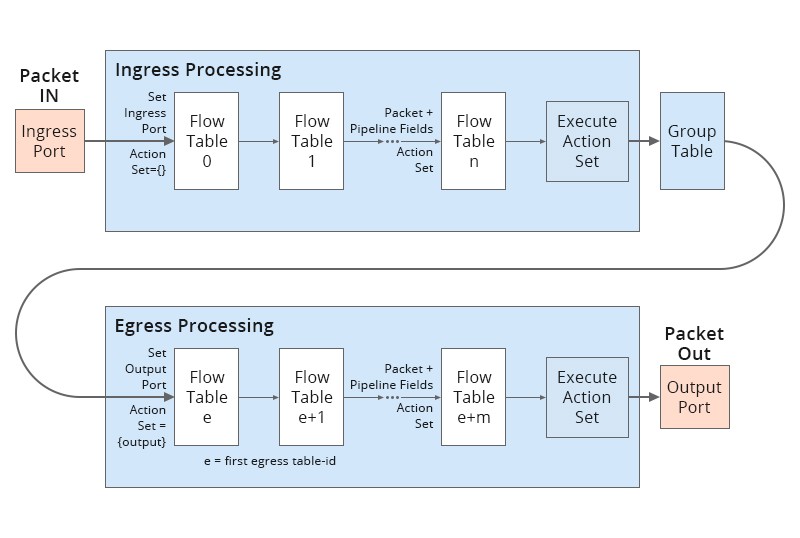
\includegraphics[width=14cm, keepaspectratio]{img/DiagramaOpenFlow}
		\caption{Diagrama de flujo de las tablas OpenFlow}
		\label{figura:DiagramaOpenFlow}
	\end{figure}
	
	Como se observa en la figura \ref{figura:DiagramaOpenFlow}, cuando un mensaje llega a un switch Open vSwitch, primero se consulta la tabla de flujo para determinar las acciones a tomar según las características del paquete. Si se encuentra una coincidencia exacta, se aplican las acciones especificadas en la regla correspondiente. En caso contrario, el mensaje puede ser dirigido a tablas adicionales, como la tabla de grupos, dependiendo de la configuración del switch. Si aún no se encuentra una coincidencia, el paquete puede ser enviado al controlador de la red para su procesamiento adicional a través del mensaje OpenFlow OFPT\_PACKET\_IN. Este proceso permite que el switch tome decisiones de enrutamiento y reenvío de manera flexible y programable.
	
	\section{Entorno de configuración y herramientas de red}
	\subsection{Mininet} 
	\label{sec:mininet}
	
	Mininet [7][8] es una plataforma de emulación de redes de código abierto que permite crear una red virtual utilizando equipos de red virtuales (switches y hosts) dentro de un entorno Linux. Proporciona un entorno de pruebas realista y escalable para experimentar, desarrollar y probar protocolos de red, aplicaciones y sistemas distribuidos.
	
	Algunas características importantes de Mininet incluyen:
	
	\begin{enumerate}
		\item 	Emulación de red: Mininet permite crear una topología de red virtual con switches Open vSwitch y hosts emulados. La topología de red y las características de los dispositivos de red se definen utilizando scripts en Python.
		\item 	Entorno aislado: Cada instancia de Mininet se ejecuta en su propio espacio de nombres de red en Linux y utiliza recursos de red virtuales, lo que proporciona un entorno aislado y seguro para realizar experimentos.
		\item 	Integración con controladores SDN: Mininet se integra fácilmente con controladores SDN como OpenDaylight, ONOS o controladores basados en Ryu. Esto permite desarrollar y probar aplicaciones y protocolos de red definidos por software utilizando un entorno emulado.
		\item 	Generación de tráfico: Mininet permite generar tráfico de red en la topología emulada. Esto es útil para evaluar el comportamiento de la red,  de los protocolos y probar la tolerancia a fallos.
		\item   Extensibilidad: Mininet es altamente extensible y se puede personalizar según las necesidades del usuario. Es posible agregar nuevos tipos de nodos de red, desarrollar controladores personalizados y utilizar módulos de extensión para ampliar su funcionalidad.
	\end{enumerate}
	
	
	Por tanto, Mininet es una herramienta muy útil para la experimentación de nuevos protocolos y arquitecturas de red, que se utiliza en el campo de la investigación en redes de ordenadores.
		
	
	
	\subsection{Ryu} 
	\label{sec:ryu}
	
	
	Ryu [11] es un framework de código abierto que está escrito en Python y proporciona una plataforma para desarrollar controladores SDN que son compatibles con el protocolo OpenFlow.
	
	Algunas características y puntos clave sobre Ryu incluyen:
	
	\begin{enumerate}
		
		\item Flexibilidad: Ryu es altamente flexible y puede utilizarse para implementar diversos algoritmos y lógicas de control en redes SDN. Los desarrolladores pueden personalizar y extender sus funcionalidades según las necesidades específicas de su red.
		
		\item Compatibilidad con OpenFlow: Ryu es compatible con múltiples versiones del protocolo OpenFlow, lo que le permite trabajar con una variedad de dispositivos y conmutadores que admiten distintas versiones del estándar.
		
		\item Programación en Python: Una característica distintiva de Ryu es que se basa en el lenguaje de programación Python. Esto facilita la escritura de controladores y aplicaciones SDN, ya que Python es conocido por su simplicidad y legibilidad.
		
		\item Aplicaciones SDN: Ryu no solo se utiliza para desarrollar un controladores básicos, sino que también puede ejecutar aplicaciones específicas SDN. Estas aplicaciones pueden implementar lógicas de red personalizadas, políticas de enrutamiento, y otras funciones.
		
		\item Comunidad Activa: Ryu es un proyecto de código abierto respaldado por una comunidad activa de desarrolladores. Esto significa que está en constante evolución y mejora, con nuevas características y correcciones de errores que se implementan de forma regular.
		
	\end{enumerate}
	
	Ryu es una herramienta utilizada para construir y personalizar controladores SDN utilizando Python y aprovechando las capacidades del protocolo OpenFlow. 
	
	\subsection{Wireshark} 
	\label{sec:wireshark}
	
	Wireshark [12] es una herramienta de análisis de tráfico de código abierto y gratuita. Permite capturar y examinar el tráfico de red en tiempo real, así como analizar y visualizar datos de capturas almacenados en ficheros de capturas. Wireshark  es ampliamente utilizado por administradores de redes, profesionales de seguridad y desarrolladores de protocolos para resolver problemas de red, realizar análisis de tráfico y depurar aplicaciones.
	
	Algunas características clave de Wireshark incluyen:
	
	\begin{enumerate}
		\item 	Captura de paquetes: Wireshark puede capturar y analizar paquetes en tiempo real de diversas interfaces de red, como Ethernet, Wi-Fi y Bluetooth. Permite seleccionar las interfaces de red específicas de las que se desea capturar el tráfico.	
		\item 	Análisis detallado: Wireshark proporciona una vista detallada de cada paquete capturado, mostrando información de los campos de los protocolos de comunicaciones como direcciones IP de origen y destino, puertos, datos de encabezado y carga útil. Permite filtrar y buscar paquetes por varios criterios, lo que facilita el análisis de tráfico específico.
		\item 	Decodificación de protocolos: Wireshark es capaz de decodificar y analizar una amplia gama de protocolos de red, incluyendo Ethernet, IP, TCP, OpenFlow entre otros. Puede reconstruir sesiones y mostrar la secuencia de intercambio de paquetes entre los dispositivos de la red.
		\item 	Estadísticas y gráficos: Wireshark proporciona estadísticas y gráficos sobre el tráfico de red capturado, por ejemplo gráficos de tiempo y el ancho de banda utilizado. Esto puede ayudar a identificar patrones de tráfico, detectar anomalías y optimizar el rendimiento de la red.
		\item   Soporte multiplataforma: Wireshark es compatible con varios sistemas operativos, incluyendo Windows, macOS y Linux. 
	\end{enumerate}
	
	
	Wireshark es una herramienta para el análisis de redes y resolución de problemas. Su interfaz intuitiva y sus capacidades de filtrado y análisis facilitan la labor de administradores de red y programadores de aplicaciones en red.
	
	%%%%%%%%%%%%%%%%%%%%%%%%%%%%%%%%%%%%%%%%%%%%%%%%%%%%%%%%%%%%%%%%%%%%%%%%%%%%%%%%
	%%%%%%%%%%%%%%%%%%%%%%%%%%%%%%%%%%%%%%%%%%%%%%%%%%%%%%%%%%%%%%%%%%%%%%%%%%%%%%%%
	% OBJETIVOS %
	%%%%%%%%%%%%%%%%%%%%%%%%%%%%%%%%%%%%%%%%%%%%%%%%%%%%%%%%%%%%%%%%%%%%%%%%%%%%%%%%
	
	\cleardoublepage % empezamos en página impar
	\chapter{Objetivos} % título del capítulo (se muestra)
	\label{chap:objetivos} % identificador del capítulo (no se muestra, es para poder referenciarlo)
	
	En este trabajo de fin de grado se va a estudiar el funcionamiento de las redes SDN
	utilizando para ello el controlador Periplus dentro
	del entorno de emulación Mininet. El objetivo
	general es conocer las redes SDN, el protocolo
	OpenFlow y el comportamiento del controlador
	Periplus en diferentes escenarios de prueba. 
	
	A continuación se detallan los objetivos concretos que permiten conseguir el objetivo general.
	\section{Subobjetivos}
	\subsection{Estudio y análisis de SDN con Mininet} % título de sección (se muestra)
	\label{sec:objetivo-mininet} % identificador de sección (no se muestra, es para poder referenciarla)
	
	Estudiar la creación de espacios de nombres de red que usa Mininet para la definición
	de los dispositivos de red que forman una determinada topología. A continuación, se estudiará Mininet para la	definición de diferentes escenarios de	red a través de la programación de scripts en Python.
		
	
	\subsection{Estudio del plano de control Periplus}
	\label{sec:objetivos-periplus}
	
	Aprender como funciona el plano de control in-band Periplus. A partir de diferentes escenarios de red con uno y varios controladores se estudiará
	el plano de control que implementa Periplus.
	
	\subsection{Realización de pruebas del plano de control Periplus y obtención de resultados}
	\label{sec:objetivos-analisis-periplus}
	
	Realizar un conjunto de pruebas para la obtención de medidas que permitan extraer conclusiones
	sobre el comportamiento de Periplus	en determinadas	situaciones como el tiempo de conexión de los switches OpenFlow al controlador o controladores en diferentes escenarios de red.
	
	
	\section{Planificación temporal}
	\label{sec:planificacion-temporal}
	
	Este trabajo se ha realizado durante más de dos años, de forma intermitente, principalmente en fines de semana y festivos. Durante todo este tiempo, hemos estado intercambiando correos, y teniendo varias reuniones de seguimiento, principalmente porque un requisito importante de este trabajo era entender perfectamente el comportamiento de Periplus.
	Además ha habido varios inconvenientes con las herramientas utilizadas que han ralentizado mucho el trabajo, con periodos de inactividad de varios meses intentando solventar los problemas.
	
	
	%%%%%%%%%%%%%%%%%%%%%%%%%%%%%%%%%%%%%%%%%%%%%%%%%%%%%%%%%%%%%%%%%%%%%%%%%%%%%%%%
	%%%%%%%%%%%%%%%%%%%%%%%%%%%%%%%%%%%%%%%%%%%%%%%%%%%%%%%%%%%%%%%%%%%%%%%%%%%%%%%%
	% INTRODUCCIÓN AL CONTEXTO %
	%%%%%%%%%%%%%%%%%%%%%%%%%%%%%%%%%%%%%%%%%%%%%%%%%%%%%%%%%%%%%%%%%%%%%%%%%%%%%%%%
	
	\cleardoublepage
		
	
	%%%%%%%%%%%%%%%%%%%%%%%%%%%%%%%%%%%%%%%%%%%%%%%%%%%%%%%%%%%%%%%%%%%%%%%%%%%%%%%%
	%%%%%%%%%%%%%%%%%%%%%%%%%%%%%%%%%%%%%%%%%%%%%%%%%%%%%%%%%%%%%%%%%%%%%%%%%%%%%%%%
	% ESTUDIO Y ANÁLISIS DE EXPERIMENTOS CON MININET %
	%%%%%%%%%%%%%%%%%%%%%%%%%%%%%%%%%%%%%%%%%%%%%%%%%%%%%%%%%%%%%%%%%%%%%%%%%%%%%%%%
	\cleardoublepage % empezamos en página impar
	\chapter{Los espacios de nombres de red en Linux  } % título del capítulo (se muestra)
	\label{chap:mininet} % identificador del capítulo (no se muestra, es para poder referenciarlo)
	
	En este trabajo de fin de grado se va a utilizar la herramienta Mininet para la emulación de diferentes
	topologías de red sobre las que probar el controlador Periplus. Mininet usa los espacios de nombres
	de red de Linux [5][9][10] para aislar el comportamiento de la red en cada uno de las máquinas emuladas. Además,
	Mininet usa Open vSwitch como dispositivo de interconexión para crear las topologías de red. En
	este capítulo se realizará un estudio de los espacios de nombres de red en Linux, su conexión
	a través de Open vSwitch y su uso en Mininet para poder entender su funcionamiento.
	
	\section{Introducción a los espacios de nombres de red en Linux}
	
	Un espacio de nombres de red es una abstracción que permite definir de forma virtual recursos de red
	aislados de los recursos físicos de la máquina. De esta forma, se pueden definir interfaces de red virtuales
	con su propia configuración diferente de los recursos reales de la máquina. A continuación se va a
	realizar un ejemplo con la configuración de dos espacios de nombres de red diferentes (''red'' y ''green'')
	conectados a través de un cable virtual Ethernet, véase figura 3.1.

	\begin{figure}[H]
		\centering
		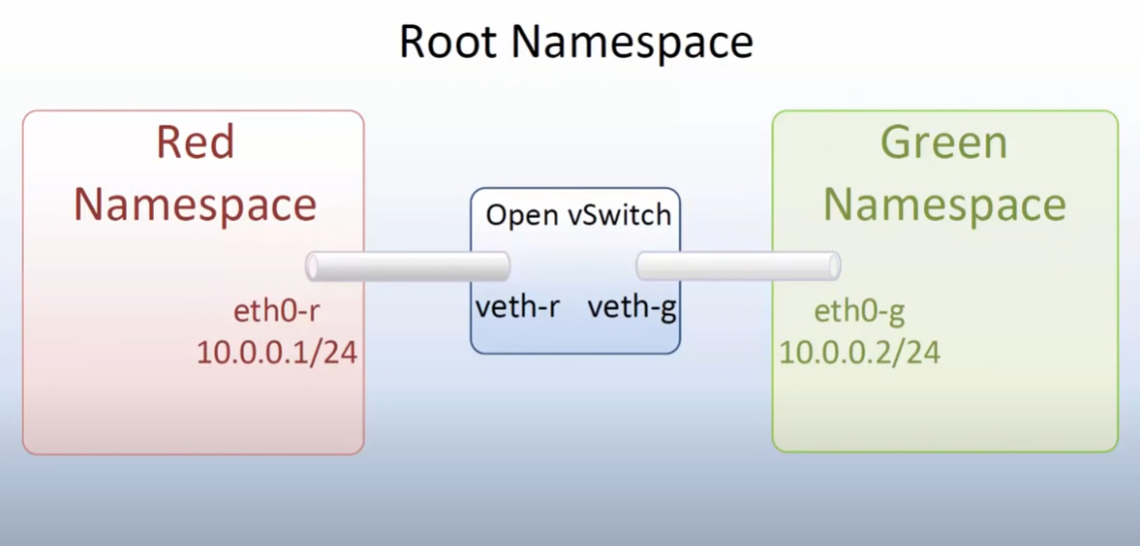
\includegraphics[width=14cm, keepaspectratio]{img/Linux namespaces}
		\caption{Creación de dos espacios de nombre de red en Linux.}
		\label{figura:linux_namespaces}
	\end{figure}
	
	Los comandos que se han utilizado para la definición de los espacios de nombres de red en Linux son:
	
	\begin{itemize}
		\item \verb*|ip link|: muestra una lista de todas las interfaces de red disponibles en el sistema, incluyendo las que están desactivadas.
		
		\item \verb*|ip address|: muestra una lista de todas las direcciones IP asociadas con las interfaces de red de un sistema.
		
		\item \verb*|ip route|: muestra la tabla de enrutamiento, que determina cómo se dirigen los paquetes de red a través de las interfaces de la máquina.
		
		\item \verb*|ip netns add red|: crea un nuevo espacio de nombres de red llamado ''red'', donde posteriormente se podrán añadir interfaces de red, tablas de enrutamiento, etc. 
		
		\item \verb*|ip netns|: muestra el listado de espacios de nombres de red, para comprobar que se han creado correctamente.
		
		\item \verb*|ip netns exec red ip link|: Ejecuta el comando ip link dentro del espacio de nombres de red llamado ''red''. 
			
		\item \verb*|ovs-vsctl add-br OVS1|: Crea un nuevo Open vSwitch que se utiliza para conectar múltiples interfaces de red virtuales y permitir la comunicación entre ellas. 
				
		\item \verb*|ip link add eth0-r type veth peer name veth-r|:  crea un cable de red virtual tipo veth (Virtual Ethernet). Este cable virtual tiene dos extremos: ''eth0-r'' y ''veth-r''.
		
		\item \verb*|ip link set eth0-r netns red|: conecta un extremo de red virtual (''eth0-r'') a un espacio de nombres de red específico (''red''). 
		
		\item \verb*|ovs-vsctl add-port OVS1 veth-r|: agrega el extremo del cable ''veth-r'' a OVS1. Como previamente se había conectado el extremo ''eth0-r'' al espacio de nombres de red ''red'', al ejecutar este comando dicho espacio de nombres quedará conectado a OVS1.
		
		\item \verb*|ip link set veth0-r up|: activa una interfaz de red virtual. En este caso, se activa la interfaz de red virtual llamada ''veth0-r'', permitiendo que pueda transmitir y recibir datos. 
		
		\item \verb*|ip netns exec red ip link set dev eth0-r up|: activa la interfaz de red ''eth0-r'' dentro del espacio de nombres de red ''red''.
		
		\item \verb*|ip netns exec red ip address add 10.0.0.1/24 dev eth0-r|: agrega una dirección IP a la interfaz de red ''eth0-r'' dentro del espacio de nombres de red llamado ''red''.
		
		
		
		
		
		
	
	\end{itemize}
	
	Utilizando estos comandos se crea un escenario simple con dos espacios de nombres de red, ''red'' y ''green'', conectados a través de un switch virtual tal y como se muestra en la figura 3.1 Cada espacio de nombres tiene su tabla de encaminamiento independiente y diferente de la tabla de encaminamiento del espacio de nombres de red raíz, que se corresponde con los recursos de la red de la máquina real.
	

	
	
	\section{Introducción a Mininet}
	
	Mininet permite la creación de espacios de nombres de red de forma más sencilla y su conexión a través
	de dispositivos Open vSwitch usando un programa en Python. Mininet ofrece una interfaz sencilla
	de programación para la creación de máquinas (que se crean con espacios de nombres de red) y su
	configuración IP, así como la creación de enlaces entre las mismas.
	Una configuración similar a la representada en la figura 3.1 se obtiene en Mininet con el siguiente
	programa en Python:
	
	 \begin{lstlisting}[caption={Ejemplo de topología simple en Mininet}, label={lst:mytopo}]
	 	from mininet.topo import Topo
	 	
	 	class MyTopo( Topo ):
	 	"Simple topology example."
	 	
	 	def __init__( self ):
	 	"Create custom topo."
	 	# Initialize topology
	 	Topo.__init__( self )
	 	
	 	# Add hosts and switches
	 	redHost = self.addHost( 'red', ip='10.0.0.1/24' )
	 	greenHost = self.addHost( 'green', ip='10.0.0.2/24' )
	 	ovs1 = self.addSwitch( 'OVS1' )
	 	
	 	# Add links
	 	self.addLink( redHost, ovs1 )
	 	self.addLink( greenHost, ovs1 )
	 	
	 	topos = { 'mytopo': ( lambda: MyTopo() ) }
	 \end{lstlisting}
	
	La función addHost crea un espacio de nombres de red denominado ''red'' al que le configura
	la dirección IP 10.0.0.1/24. Esta misma función se utiliza para crear el espacio de nombres de
	red llamado ''green'' con la dirección IP 10.0.0.2/24.
	La función addSwitch crea un Open vSwitch llamado ''OVS1''. A continuación crea cables virtuales
	para conectar el Open vSwitch con los espacios de nombres ''red'' y ''green'' a través de la función
	addLink.
	
	Como se ha podido demostrar, el uso de Mininet permite programar de forma sencilla
	topologías de red gracias a la interfaz de programación en Python. Configurar manualmente
	los espacios de nombres de red sería muy complicado cuando se desean escenarios con
	muchos dispositivos conectados entre ellos. Por este motivo, Mininet se usa como herramienta
	para la emulación de topologías de red en las que probar protocolos de comunicaciones.
	
	
	
	%%%%%%%%%%%%%%%%%%%%%%%%%%%%%%%%%%%%%%%%%%%%%%%%%%%%%%%%%%%%%%%%%%%%%%%%%%%%%%%%
	%%%%%%%%%%%%%%%%%%%%%%%%%%%%%%%%%%%%%%%%%%%%%%%%%%%%%%%%%%%%%%%%%%%%%%%%%%%%%%%%
	% ESTUDIO Y ANÁLISIS DEL PLANO DE CONTROL EN BANDA PERIPLUS %
	%%%%%%%%%%%%%%%%%%%%%%%%%%%%%%%%%%%%%%%%%%%%%%%%%%%%%%%%%%%%%%%%%%%%%%%%%%%%%%%%
	\cleardoublepage % empezamos en página impar
	\chapter{Estudio y análisis del plano de control Periplus} % título del capítulo (se muestra)
	\label{chap:periplus} % identificador del capítulo (no se muestra, es para poder referenciarlo)
	
	Este trabajo de fin de grado se centra principalmente en el plano de control in-band que genera el controlador Periplus. Este plano de control está desarrollado en Python por el Grupo de Investigación de Alto Rendimiento en Tecnologías de la Información y Comunicaciones para el Desarrollo Humano de la Universidad Rey Juan Carlos. Periplus es un controlador in-band, es decir, que utiliza la misma infraestructura tanto para el plano de datos como para el plano de control. Partiendo de una configuración inicial mínima, los switches OpenFlow deben descubrir donde
	se encuentra el controlador para establecer una conexión TCP que permita definir la sesión
	OpenFlow. Una vez establecida esa sesión Periplus podrá instalar en los switches la configuración
	necesaria para el plano de control.	Para ello, Periplus utiliza mecanismos como Proxy ARP y Anycast que facilitan el descubrimiento de la máquina en la que se encuentra el controlador.
	
	Periplus busca aumentar la robustez del plano de control permitiendo que los switches reaccionen rápidamente a fallos en enlaces y switches sin necesidad de esperar nuevas instrucciones del controlador, ya que los propios mensajes contienen información de las posibles rutas alternativas cuando falle un enlace.
	Además, se minimiza la cantidad de flujos almacenados en los switches que admiten el plano de control, ya que la información de enrutamiento no se almacena en los switches, sino en los caminos que van encapsulados en los paquetes intercambiados en el plano de control.
	
	
	\section{Inicialización de la Comunicación Controlador-Switch}
	
	El proceso de inicialización de la comunicación entre un controlador SDN y los switches es esencial para garantizar el funcionamiento coordinado de la red. Este proceso incluye varias etapas clave, cada una de las cuales es crucial para establecer una red operativa y gestionable. A continuación, se presenta una descripción detallada de este proceso:
	
	\subsection{Descubrimiento del Controlador}
	
	Al iniciar los switches, estos deben establecer una conexión TCP con el controlador SDN. Esta conexión se utilizará para establecer la sesión OpenFlow entre cada switch y el controlador.
		Para enviar mensajes al controlador, el switch primero necesita conocer su dirección Ethernet. El primer mensaje que un switch enviará será una solicitud ARP para obtener la dirección Ethernet del nodo donde está el controlador.

	Si el switch que está arrancando está directamente conectado al controlador o a otro
	switch que ya está gestionado por el controlador, el nuevo switch recibirá la respuesta
	de ARP que le permitirá conectarse 	con el controlador. Si no fuera así, el nuevo switch
	deberá esperar 	a que un  switch vecino	esté gestionado	por el	controlador para establecer la conexión TCP.
	
	\subsection{Establecimiento de la Sesión OpenFlow}
	
	
	El controlador y cada uno de los switches establecen una sesión OpenFlow para intercambiar mensajes de configuración. Esto incluye la configuración inicial de los flujos OpenFlow que definen el comportamiento básico de los switches.

	
	\subsection{Intercambio inicial de características}
	El controlador y los switches intercambian un conjunto de mensajes OpenFlow:
	\begin{itemize}
		\item \textbf{Reporte de características}: Los switches informan al controlador sobre sus características, como el número de puertos y características específicas del hardware.
		\item \textbf{Evaluación por el Controlador}: El controlador utiliza esta información para optimizar las decisiones de enrutamiento y gestión de flujos.
	\end{itemize}
	
	El controlador va obteniendo la información de la topología completa de la red y podrá calcular los caminos más cortos entre cada switch y el controlador y viceversa, aplicando Dijkstra.
	
	\subsection{Instalación de Flujos para encaminamiento}
	A partir de la información de encaminamiento calculada por el controlador se realizarán las siguientes funciones:
	\begin{itemize}
		\item \textbf{Definición de Flujos Básicos}: El controlador envía flujos iniciales a los switches, que permiten definir el comportamiento del switch cuando éste tiene que enviar un mensaje al controlador o cuando el switch tiene que reenviar un mensaje a un determinado destino.
		\item \textbf{Implementación en los Switches}: Los switches aplican estas reglas en sus tablas de flujo, para implementar la función de encaminamiento.
	\end{itemize}
	
	\subsection{Monitorización de la red}
		El controlador vigila el funcionamiento la red y ajusta los flujos instalados en los switches si se producen cambios en la red.
		Ante la aparición de nuevos switches o problemas en los enlaces, el controlador aplicará nuevamente Dijkstra sobre la topología modificada y recalculará los caminos que permitan la comunicación entre dispositivos.
	
	\section{Sesión OpenFlow}
	Vamos a describir el intercambio de mensajes OpenFlow cuando se arranca un escenario desde cero. Este proceso implica la conexión inicial entre el controlador y el switch, así como la configuración de reglas de flujo. 
	
	\begin{itemize}
		\item Inicio del Controlador y Switches:
		\begin{itemize}
			\item El controlador SDN y los switches OpenFlow se inician.
			\item Los switches establecen conexiones TCP con el controlador.
		\end{itemize}
		
		\item Comunicación Inicial:
		\begin{itemize}
			\item Los switches envían mensajes OFPT\_HELLO para iniciar la comunicación con el controlador.
			\item El controlador responde con mensajes OFPT\_HELLO.
		\end{itemize}
		
		\item Negociación de Características (Feature Negotiation):
		\begin{itemize}
			\item El controlador envía mensajes OFPT\_FEATURES\_REQUEST
			a cada switch para obtener información sobre sus características y capacidades.
			\item Cada switch responde con mensajes OFPT\_FEATURES\_REPLY, proporcionando detalles como
			el número de puertos y las capacidades compatibles.
		\end{itemize}
		
		\item Configuración de flujos iniciales:
		\begin{itemize}
			\item El controlador envía mensajes OFPT\_FLOW\_MOD a los switches para configurar reglas
			de flujo iniciales. Estas reglas especifican cómo se deben manejar ciertos tipos de tráfico en la red.
			\item Los switches ejecutarán las acciones definidas en estos flujos para implementar el encaminamiento decidido por el controlador. 
		\end{itemize}
	
		
		\item Encaminamiento de Paquetes en los switches:
		\begin{itemize}
			\item Cuando un switch recibe un paquete, verifica las reglas de flujo en su tabla de
			flujo para determinar que acciones debe ejecutar para encaminarlo.
			\item Si no hay reglas coincidentes, el switch puede enviar el paquete al controlador
			mediante un mensaje OFPT\_PACKET\_IN. Estos paquetes permiten que el controlador configure nuevas reglas que instruyan al switch para gestionar este tipo de paquetes.
		\end{itemize}
		
		\item Sondeo de Conexión:
		\sloppy
		\begin{itemize}
			\item El controlador puede enviar mensajes OFPT\_ECHO\_REQUEST para realizar pruebas de sondeo de la conexión. Estas pruebas muestran si ha habido algún problema de conexión en alguno de los switches, si no se obtiene respuesta en un tiempo relativamente corto.
		\item Cada switch responde a los mensajes OFPT\_ECHO\_REQUEST con mensajes OFPT\_ECHO\_REPLY.
		\end{itemize}
		\fussy
		
		\item Actualizaciones de Flujos:
		\begin{itemize}
			\item A medida que cambian las condiciones de la red o se producen eventos específicos,
			el controlador puede enviar nuevos mensajes OFPT\_FLOW\_MOD adicionales para actualizar
			dinámicamente las reglas de flujo en los switches que reflejen los cambios que se han producido en la red.
		\end{itemize}
	\end{itemize}
	
	\section{Encaminamiento Basado en Origen}
	Periplus utiliza un modelo de encaminamiento basado en origen. Los nodos que se comunican insertan en los mensajes el camino que deben seguir para llegar al destino, y los nodos intermedios extraen esta información para reenviar los mensajes. El controlador ha calculado un camino principal y
	posibles caminos alternativos desde cada nodo al controlador y viceversa. Los flujos que instala el controlador en los switches
	permiten insertar estos	caminos	en los mensajes	que	envía cada switch.
	
	Para calcular los caminos, el controlador construye un árbol virtual con la raíz en el nodo origen. Este árbol permite calcular los caminos más cortos para la comunicación entre el controlador y los switches.
		
	La comunicación entre los nodos ya gestionados y el controlador se lleva a cabo mediante un proceso de encaminamiento en origen, diseñado para establecer una comunicación tolerante a fallos en una red definida por software. 
	
	El controlador genera un ''grafo'' que representa la ruta completa que un paquete debe seguir para llegar desde un switch hasta el controlador, o viceversa, y el grafo se inserta en cada mensaje que se intercambian los switches y el controlador. Así, cada paquete transporta consigo la información necesaria para su encaminamiento a lo largo de la red utilizando los protocolos existentes.
	
	El controlador configura los flujos OpenFlow en cada switch gestionado para que incluyan estos grafos en una cabecera adicional de los paquetes. Esto implica definir reglas específicas en los switches para interpretar y procesar adecuadamente la información del grafo contenida en las cabeceras adicionales de los paquetes. De esta manera, los switches intermedios interpretan la información de enrutamiento que se incluye en los mensajes.
	
	Para transmitir esta información de encaminamiento, se utiliza la cabecera NSH (Network Service Headers) que se situa entre las cabeceras de nivel 2 y 3. Aunque el protocolo NSH se utiliza típicamente para la comunicación entre controladores SDN, en este contexto se utiliza con un objetivo diferente, como un contenedor de información de encaminamiento. Esta adaptación permite transportar los grafos de encaminamiento a lo largo de la red.
	
	El grafo incluye un camino primario codificado como una lista de puertos de salida de los switches en el camino, además de caminos alternativos utilizando la misma codificación.
	
	A continuación se muestra un ejemplo de codificación del grafo.
	
	\begin{figure}[H]
		\centering
		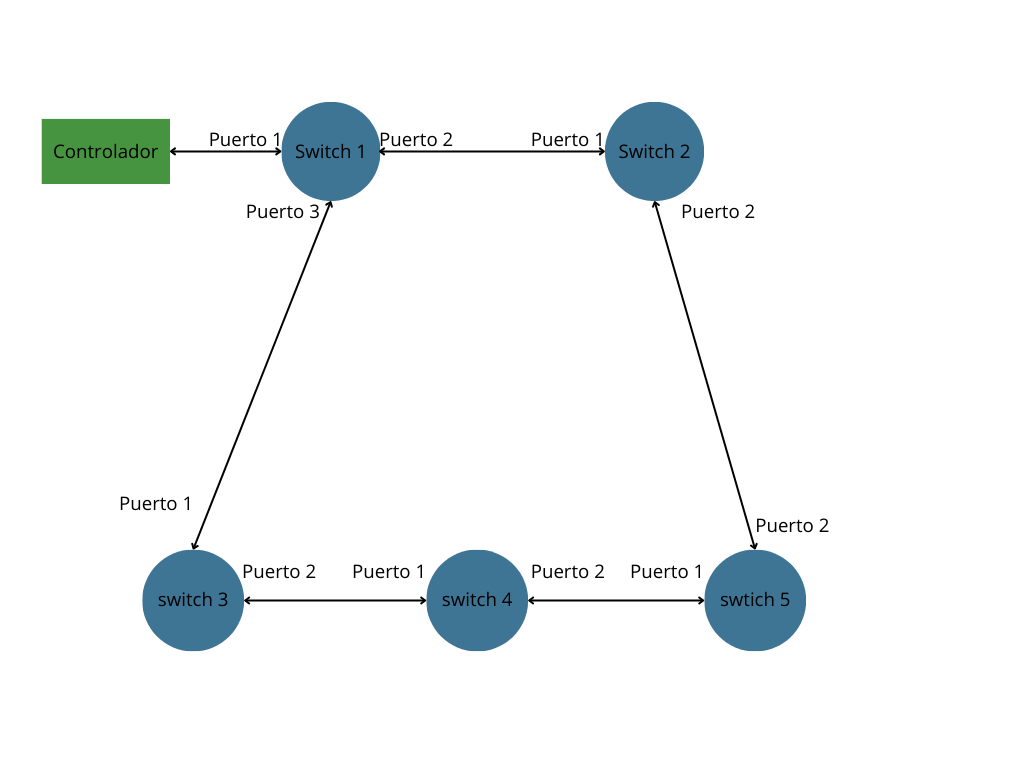
\includegraphics[width=16cm, keepaspectratio]{img/Ejemplo Periplus 1}
		\caption{Escenario formado por 5 switches y un nodo controlador.}
		\label{figura:PeriplusEj1}
	\end{figure}
	
	Supongamos que tenemos un escenario simple con 5 switches y un controlador como el mostrado en la Figura \ref{figura:PeriplusEj1}. La comunicación entre el controlador y el switch 5 se puede realizar a través de 2 caminos posibles, uno más corto siguiendo la ruta controlador $\rightarrow$ s1 $\rightarrow$ s2 $\rightarrow$ s5 y otro más largo a través de controlador $\rightarrow$ s1 $\rightarrow$ s3 $\rightarrow$ s4 $\rightarrow$ s5. 
	
	El mensaje que sale de un nodo llevará en la cabecera NSH los números de puerto de salida de cada
	switch que indican el camino que debe llevar el mensaje desde el origen al destino.
	
	\begin{figure}[H]
		\centering
		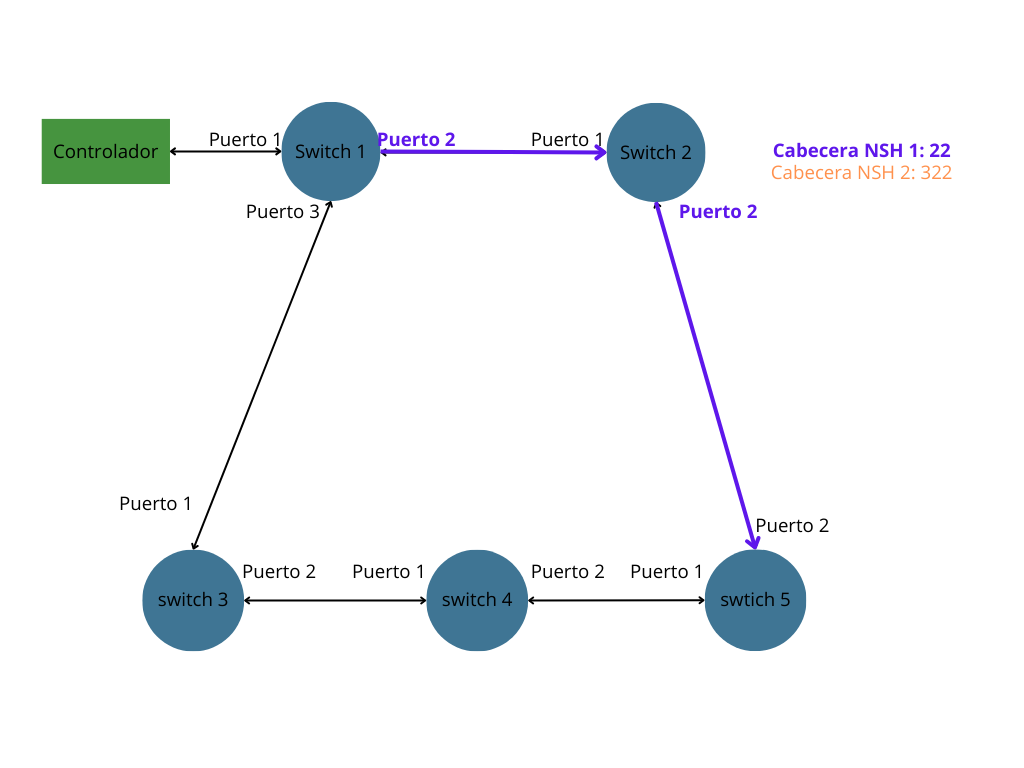
\includegraphics[width=16cm, keepaspectratio]{img/Ejemplo Periplus 2}
		\caption{Comunicación desde el controlador al switch 5.}
		\label{figura:PeriplusEj2}
	\end{figure}
	
	En el ejemplo que se muestra en la figura \ref{figura:PeriplusEj2}, el controlador desea enviar un mensaje
	al switch 5. El mensaje que enviará el controlador y que podrá capturarse en el enlace que une el
	controlador con el switch 1 debe llevar en la cabecera NSH el grafo que contiene
	los puertos de salida en cada switch para llegar al switch 5. En este caso,
	el grafo debe ser 22. Cuando el mensaje llegue al switch 1, éste debe eliminar del
	grafo el puerto por donde lo envía (puerto 2) y
	enviarlo a través de dicho puerto (puerto 2). Cuando el mensaje alcance el
	switch 2, éste debe eliminar del grafo el puerto por donde lo envía (puerto 2) y enviarlo
	a través de dicho puerto (puerto 2). De esta forma el mensaje llegará a
	su destino.
	Adicionalmente, el mensaje que envíe el controlador contendrá también un camino alternativo,
	por si se produce algún fallo en el camino principal. El camino alternativo en este caso queda
	definido por el grafo 322. Es decir, desde el switch 1 se envía a través del puerto 3, al llegar al
	switch 3 se envía a través del puerto 2 y al llegar al switch 4 se envía a través del puerto 2.


	\begin{figure}[H]
		\centering
		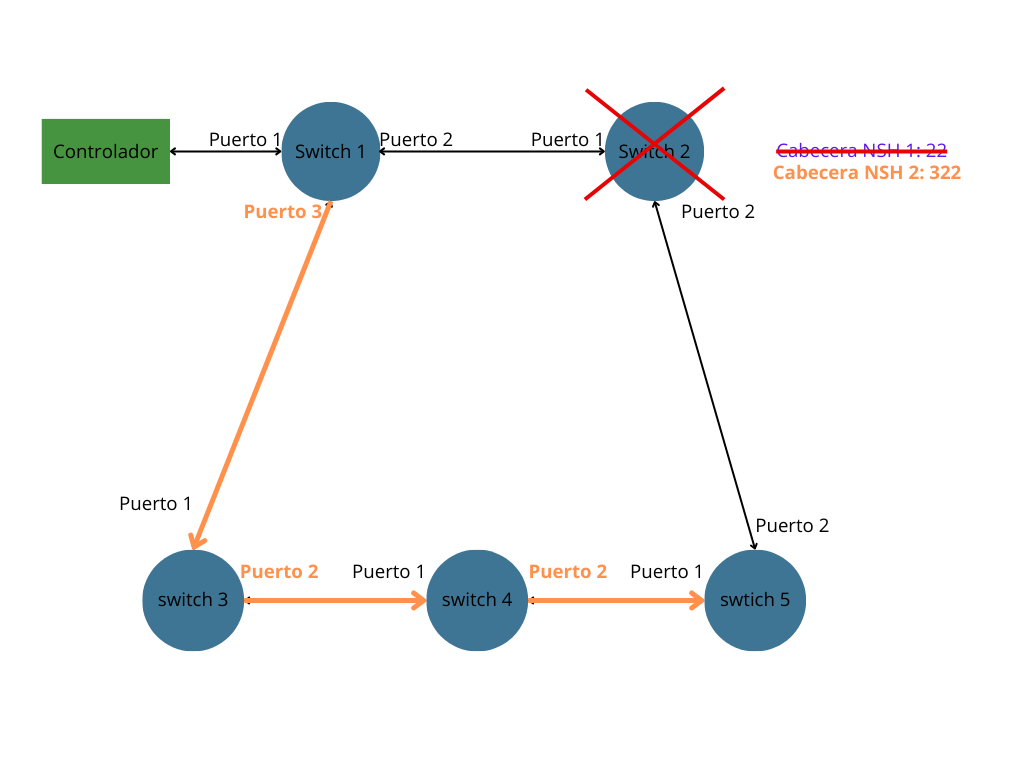
\includegraphics[width=16cm, keepaspectratio]{img/Ejemplo Periplus 3}
		\caption{Escenario de Ejemplo 3}
		\label{figura:PeriplusEj3}
	\end{figure}
	
	En el caso de que el switch 2 estuviera desactivado, el switch 1 elegiría el camino alternativo, como se muestra en la Figura \ref{figura:PeriplusEj3} marcado en color naranja.
	

	\section{Gestión de los switches: Tablas OpenFlow}
	
	En el proceso de gestión de los switches por parte del controlador en una red definida por software, se configuran las tablas OpenFlow en cada switch para garantizar un enrutamiento eficiente del tráfico de red. Estas tablas, divididas en varios niveles, determinan el flujo de los paquetes a través de la red.
	
	La primera tabla, denominada Tabla 0, es la primera en ser consultada por los paquetes entrantes. Su función principal es verificar si hay más saltos en el camino principal del paquete y, en caso afirmativo, almacenar la información del próximo salto en un registro específico. A continuación, el paquete se reenvía a las Tablas 1 y 2 para un procesamiento adicional.
	
	La Tabla 1 se utilizaba en una implementación alternativa del controlador para la detección de puertos inactivos, pero en la implementación actual está vacía. Por otro lado, la Tabla 2 asigna el paquete a una ''tabla de grupo''. Esta tabla de grupo se encarga de detectar la actividad de los puertos mediante mensajes del protocolo Bidirectional Forwarding Detection (BFD) y, en función de ello, enviar el paquete a la Tabla 11 si el camino está activo, o continuar con el procesamiento en la Tabla 3.
	
	La Tabla 11, utilizada desde la tabla de grupo, almacena el puerto de salida activo en un registro y envía el paquete a la Tabla 3. Aquí, se desencapsula la cabecera NSH de los paquetes y se elimina el puerto de salida del grafo. Si el puerto está activo, el paquete se envía por ese puerto; de lo contrario, se consulta si existe un camino alternativo.
	
	Las Tablas 4 y 5 se utilizan en caso de que exista camino alternativo. Se elimina el camino principal de la cabecera NSH para sustituirlo por el camino alternativo almacenado en la siguiente cabecera NSH. A continuación, el paquete se reenvía a la Tabla 0 para su procesamiento posterior.
	
	 
	%%%%%%%%%%%%%%%%%%%%%%%%%%%%%%%%%%%%%%%%%%%%%%%%%%%%%%%%%%%%%%%%%%%%%%%%%%%%%%%%
	%%%%%%%%%%%%%%%%%%%%%%%%%%%%%%%%%%%%%%%%%%%%%%%%%%%%%%%%%%%%%%%%%%%%%%%%%%%%%%%%
	% EXPERIMENTOS Y VALIDACIÓN %
	%%%%%%%%%%%%%%%%%%%%%%%%%%%%%%%%%%%%%%%%%%%%%%%%%%%%%%%%%%%%%%%%%%%%%%%%%%%%%%%%
	
	\clearpage
	\chapter{Experimentos con Periplus en diferentes escenarios}
	\label{chap:experimentos}
	
 	A lo largo de este capítulo se van a realizar experimentos de arranque de Periplus en 4 escenarios de red en los que configuraremos el uso de un controlador o varios controladores. Posteriormente se compararán los resultados en cuanto al tiempo de conexión de los switches con el o los controladores, analizando así cómo afecta a un escenario el añadir nuevos controladores.%
	 
	Para ello, se realizará una recogida de datos respecto a los tiempos de conexión de un conjunto de switches a sus controladores y se mostrarán gráficamente los resultados: 
	
	
	\begin{itemize}
		\item Se recogerá el tiempo que tardan en conectarse todos los switches. Con esta información podemos saber el tiempo que tarda el escenario en estar operativo. Esta medida es muy útil, principalmente para comparar tiempos entre escenarios con uno y varios controladores.
		
		\item Se recogerá la información de qué switches tiene conectado cada controlador. Esta medida mostrará cómo funcionan los escenarios con multicontrolador, indicando el reparto de switches por controlador. Se observará además que, como era de esperar, a mayor cercanía del controlador, más posibilidades de estar conectado a dicho controlador.
		
		\item Se recogerá el camino que ha seguido cada switch para conectarse a su controlador. Con este estudio podemos ver en qué orden se han ido conectando los switches.
		
	\end{itemize}
 	
 	\clearpage
 	\section{Escenario 1}
 	
 	En la figura \ref{figura:escenario1-1c} se muestra la conexión de un controlador
	ejecutándose en una máquina que tiene configurada la dirección
 	IP 10.0.0.1 y 8 switches. Junto a la interfaz Ethernet de cada switch
 	se muestra el número de puerto al que se corresponde dicha interfaz.
 	Los switches tienen configuradas las direcciones IP que se muestranen el lado izquierdo de la figura \ref{figura:escenario1-1c}:
 	
 	\vspace*{-18pt}
 	%Figura Escenario 1 con 1 controlador
 	\begin{figure}[H]
 		\centering
 		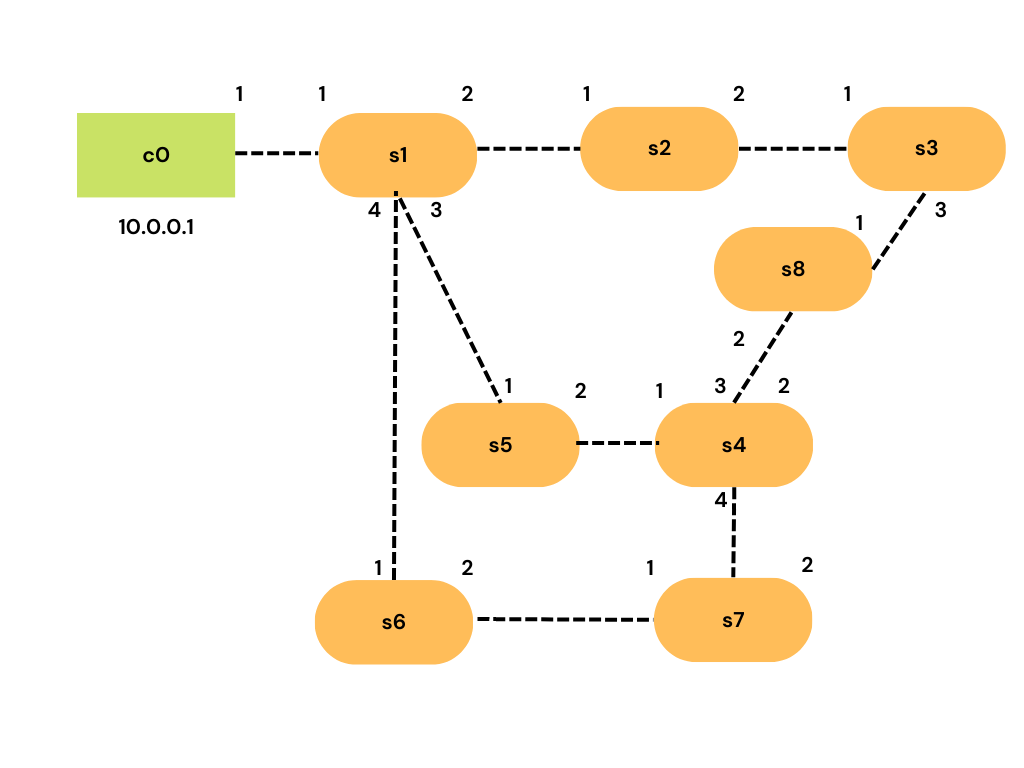
\includegraphics[width=16cm, keepaspectratio]{img/escenario1-1}
 		\caption{Escenario 1: un controlador y 8 switches.}
 		\label{figura:escenario1-1c}
 	\end{figure}
 	
 	En la figura \ref{figura:escenario1-explicado} podemos ver en rojo, el número de saltos de distancia desde cada switch al controlador, siendo el más lejano el switch s8, con una distancia o diámetro de la red igual a 4.
 	%Figura Escenario 1 con 1 controlador explicado
 	\begin{figure}[H]
 		\centering
 		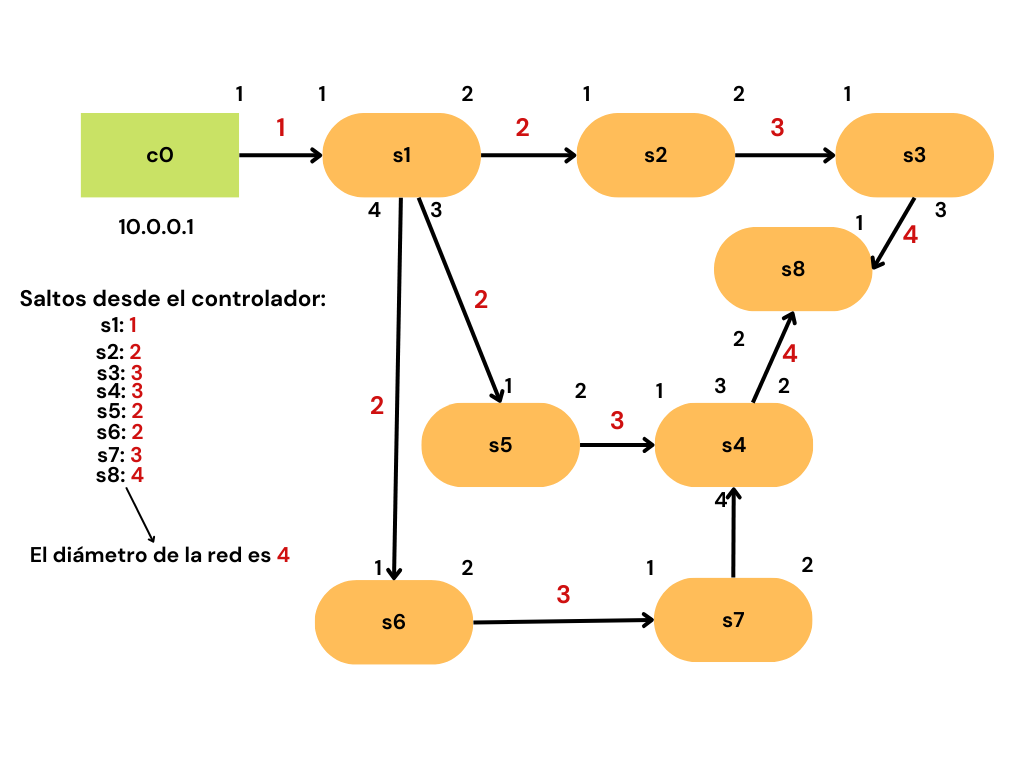
\includegraphics[width=12cm, keepaspectratio]{img/escenario1-explicado}
 		\caption{Escenario 1: diámetro de la red.}
 		\label{figura:escenario1-explicado}
 		\vspace{-18pt}
 	\end{figure}
 	
 	En la figura \ref{figura:escenario1-2c} se muestra la misma topología de la figura \ref{figura:escenario1-1c} pero con 2 controladores: c0 y c1. Ambos controladores tienen configurada la misma dirección IP para provocar que los switches se conecten al controlador más cercano. Los switches no saben a cuál de los controladores se están conectando porque establecen una conexión TCP con la dirección IP 10.0.0.1, que es la misma para ambos controladores.
 	
 	%Figura Escenario 1 con 2 controladores
 	\begin{figure}[H]
 		\centering
 		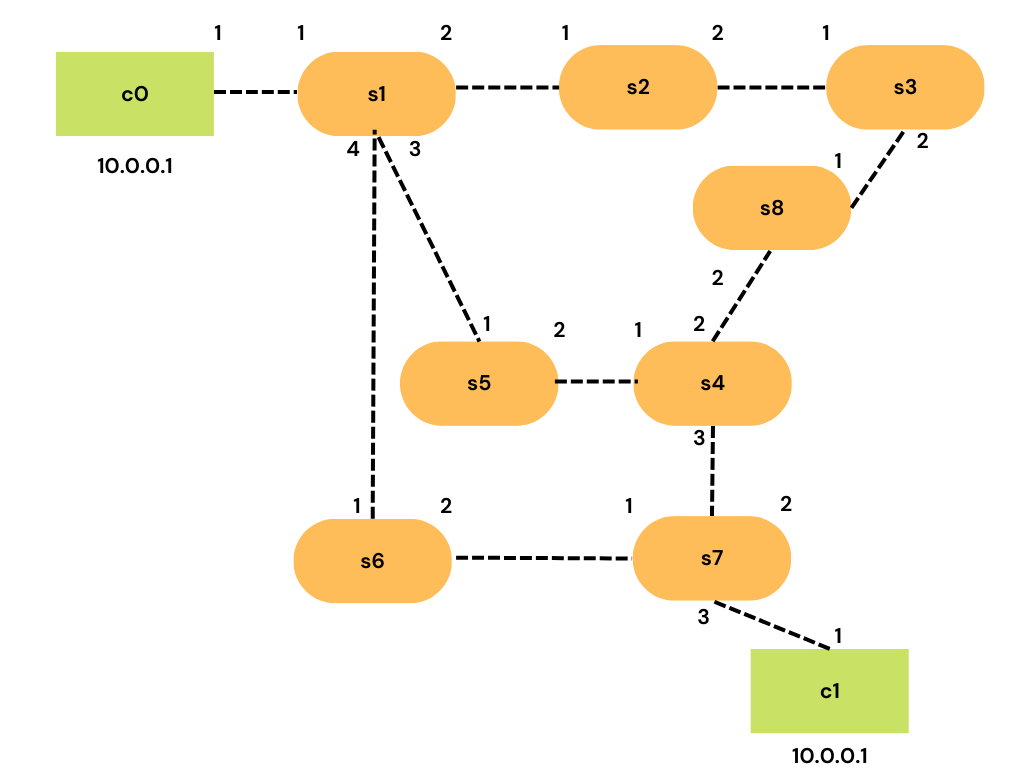
\includegraphics[width=12cm, keepaspectratio]{img/escenario1-2}
 		\caption{Escenario 1: 2 controladores y 8 switches.}
 		\label{figura:escenario1-2c}
 		\vspace{-18pt}
 	\end{figure}
 	
 	 Al añadir un segundo controlador en el otro extremo del escenario, los switches deberían conectarse al controlador más cercano en número de saltos. Por tanto, los switches	 s1, s2, s3 y s5 deberían conectarse al controlador c0 y los switches s7, s4 y s6 al controlador c1. El switch
 	 s8 está a igual distancia de ambos controladores, por lo que podría conectarse tanto a c0 como a c1.
 	 
 	 A continuación se han realizado 10 medidas diferentes para ver el tiempo que tardan todos los switches en estar gestionados por un controlador en el escenario 1, tanto con con 1 controlador, como en el de 2 controladores.
 	
 En la figura \ref{figura:comparativabucle4} se muestran los resultados obtenidos para los 10 intentos realizados en el arranque del escenario 1. La agregación de nuevos controladores a un escenario reducirá los tiempos máximos de conexión. La media de la mejora en el tiempo de conexión de todos los switches en este escenario es de 0.0546 segundos, siendo esto una mejora del 14.59 \% al añadir un controlador adicional al escenario. 
 	Estos resultados coinciden con lo que se esperaba previamente, ya que hay una mejoría, pero no es demasiado grande con respecto al mismo escenario con un solo controlador.
 	
 	%Figura comparativa de tiempos en el primer escenario
 	\begin{figure}[H]
 		\centering
 		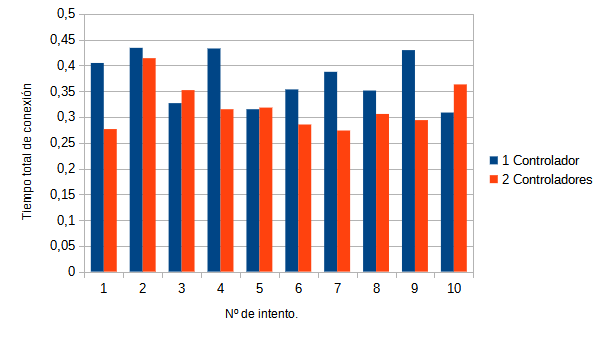
\includegraphics[width=16cm, keepaspectratio]{img/comparativabucle4}
 		\caption{Tiempo que tardan todos los switches del escenario 1 en estar gestionados por un controlador.}
 		\label{figura:comparativabucle4}
 	\end{figure}
 	
 	%Figura comparativa de medias en el primer escenario
 	\begin{figure}[H]
 		\centering
 		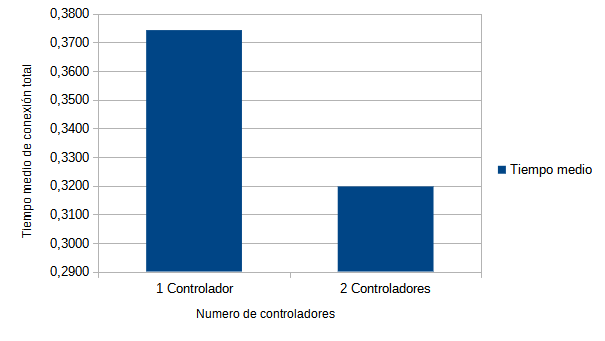
\includegraphics[width=12cm, keepaspectratio]{img/comparativamediasbucle}
 		\caption{Comparativa de media de tiempos en conseguir que todos los switches del escenario 1 estén gestionados por un controlador}
 		\label{figura:mediabucle4}
 	\end{figure}
 	
 	Como vemos en la figura \ref{fig:mediana} y la figura \ref{fig:varianza} , también hay bastante diferencia en la mediana y la varianza. Al haber 2 controladores, es difícil que haya tiempos muy altos, de ahí que se reduzca la mediana y la varianza.

 	 
 	 \begin{figure}[H]
 	 	\centering
 	 	\begin{minipage}[b]{0.45\textwidth}
 	 		\centering
 	 		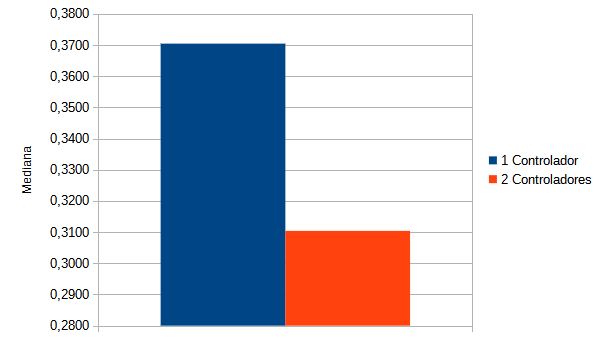
\includegraphics[width=\textwidth]{img/comparativamedianabucle.png}
 	 		\caption{Comparativa de medianas en conseguir que todos los switches del escenario 1 estén gestionados por un controlador.}
 	 		\label{fig:mediana}
 	 	\end{minipage}
 	 	\hfill
 	 	\begin{minipage}[b]{0.45\textwidth}
 	 		\centering
 	 		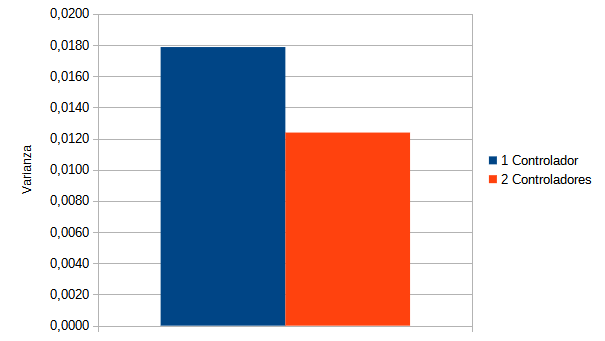
\includegraphics[width=\textwidth]{img/comparativavarianzabucle.png}
 	 		\caption{Comparativa de varianza en conseguir que todos los switches del escenario 1 estén gestionados por un controlador.}
 	 		\label{fig:varianza}
 	 	\end{minipage}
 	 \end{figure}
 	 	
 
 	
 	Con el objetivo de ilustrar cómo cambia el escenario al añadir un controlador adicional, se van a comparar los dos experimentos analizando como se han ido conectando los switches paso a paso en los 10 intentos realizados.
 	
 	Para el caso de 1 controlador, los switches se han ido conectando según el orden mostrado en la figura \ref{figura:escenario1_1c_1}:
 	
 	\begin{figure}[H]
 		\centering
 		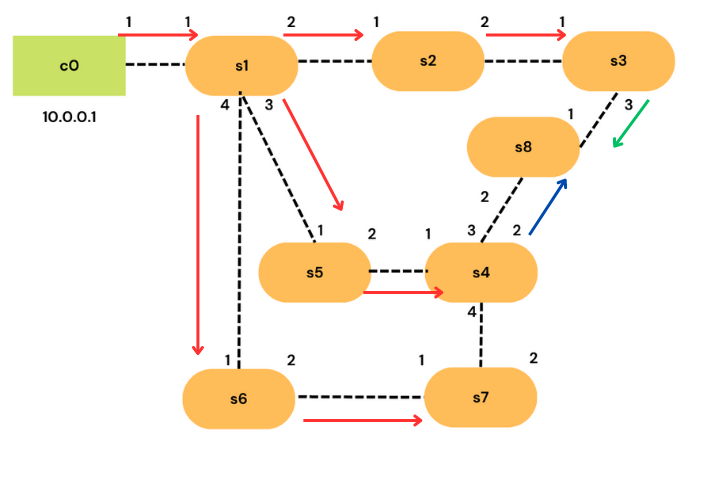
\includegraphics[width=16cm, keepaspectratio]{img/rutasEscenario1-1c}
 		\caption{Orden de conexión de los switches. El color rojo indica que todos los switches salvo s8 se han conectado de la misma forma en las 10 ejecuciones siguiendo el árbol de conexión de las flechas rojas.}
 		\label{figura:escenario1_1c_1}
 	\end{figure}
 	
 	Las diferencias entre las ejecuciones se encuentran en el switch s8 que puede alcanzar
 	el controlador con el mismo coste (en número de saltos) a través de 2 caminos diferentes.
 	En las pruebas realizadas, en 2 ejecuciones s8 se conectó a través de s3 (camino verde
 	en la figura \ref{figura:escenario1_1c_1})	y en 8 ejecuciones s8 se conectó a través de s4 (camino	azul).
 	
 	Para el caso de 2 controladores, los resultados son muy variados, como se muestra en las figuras de \ref{figura:8} a \ref{figura:16}:
 	
 	\begin{figure}[H]
 		\centering
 		\begin{minipage}[b]{0.35\textwidth}
 			\centering
 			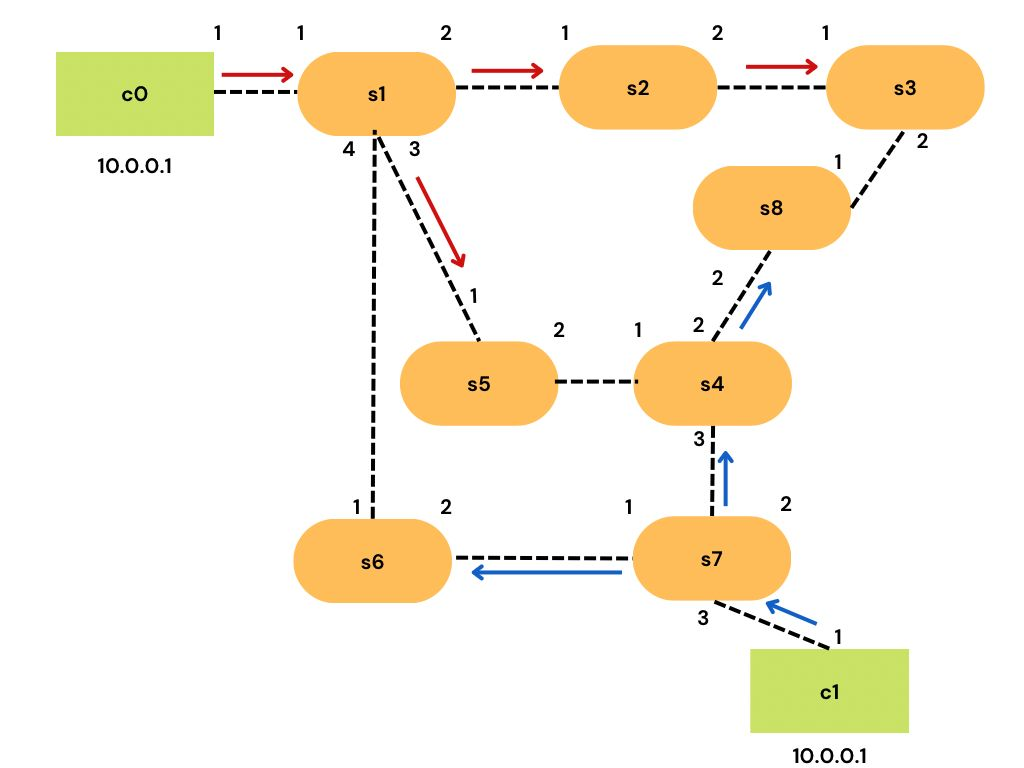
\includegraphics[width=\textwidth]{img/escenario1_2c_1}
 			\caption{Orden de conexión de los experimentos 1, 4}
 			\label{figura:8}
 		\end{minipage}
 		\hfill
 		\begin{minipage}[b]{0.35\textwidth}
 			\centering
 			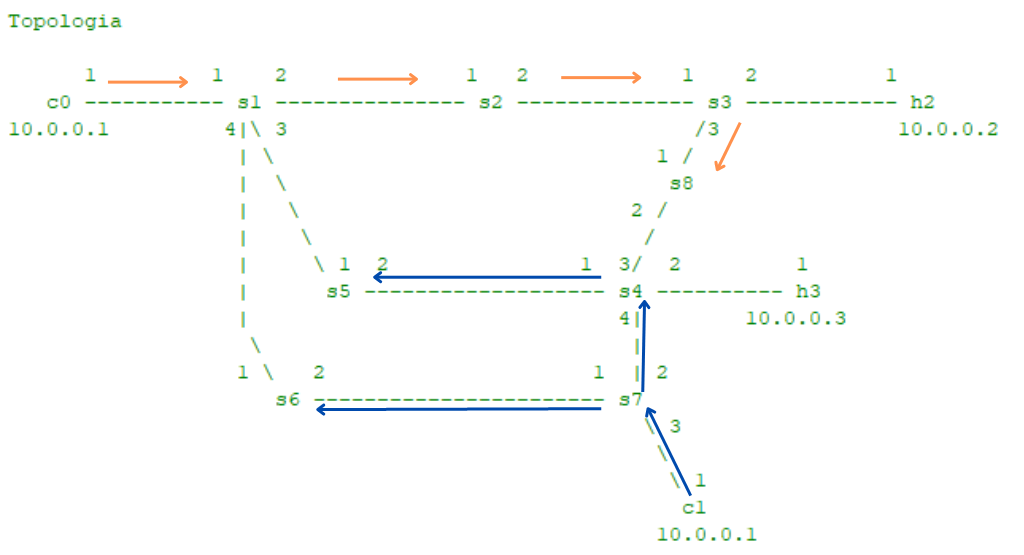
\includegraphics[width=\textwidth]{img/escenario1_2c_2}
 			\caption{Orden de conexión de los experimentos 2, 9}
 		\end{minipage}
 		
 		\vspace{10pt} % Ajusta el espacio vertical entre las filas
 		
 		\begin{minipage}[b]{0.35\textwidth}
 			\centering
 			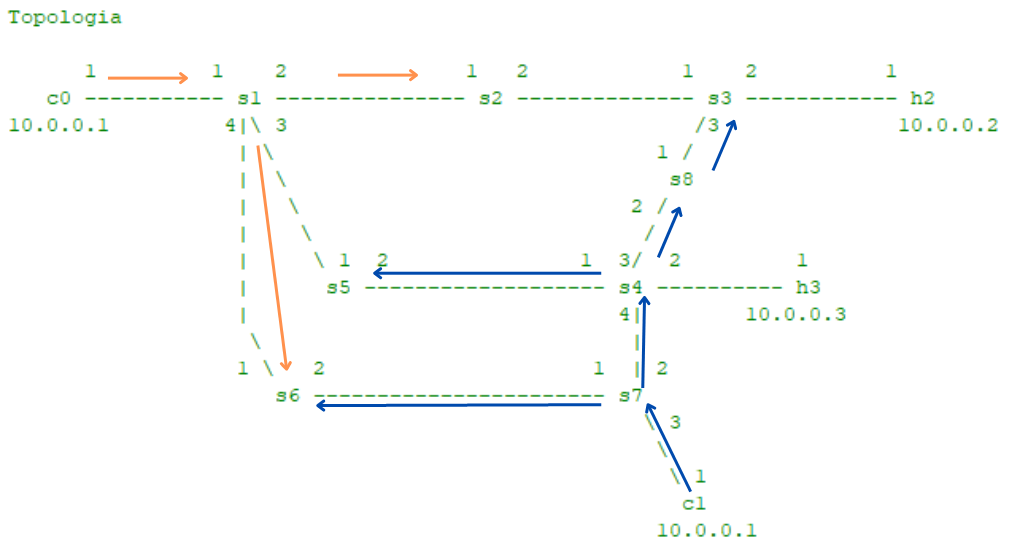
\includegraphics[width=\textwidth]{img/escenario1_2c_3}
 			\caption{Orden de conexión del experimento 3}
 		\end{minipage}
 		\hfill
 		\begin{minipage}[b]{0.35\textwidth}
 			\centering
 			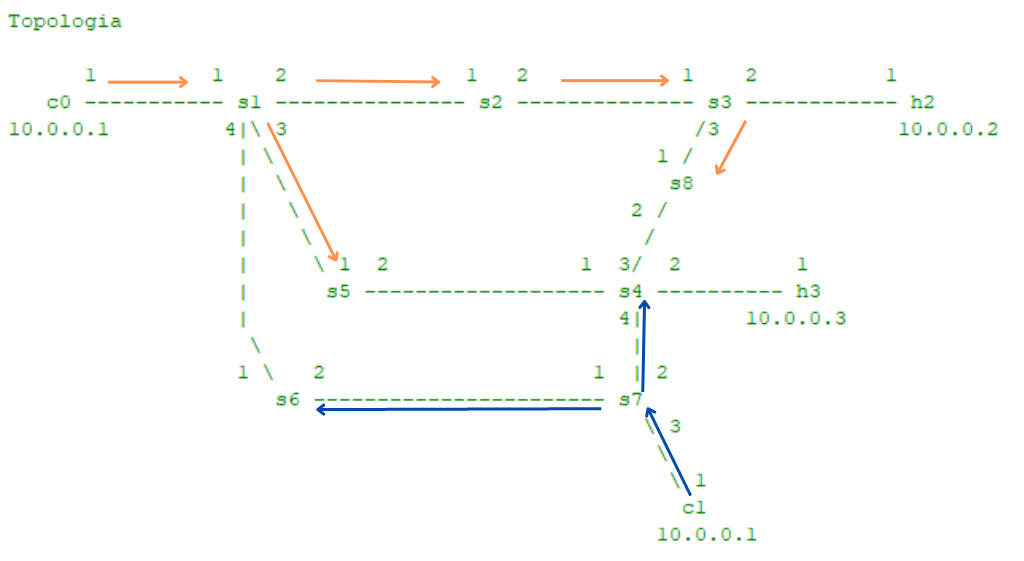
\includegraphics[width=\textwidth]{img/escenario1_2c_4}
 			\caption{Orden de conexión del experimento 5}
 		\end{minipage}
 		
 		\vspace{10pt} % Ajusta el espacio vertical entre las filas
 		
 		\begin{minipage}[b]{0.35\textwidth}
 			\centering
 			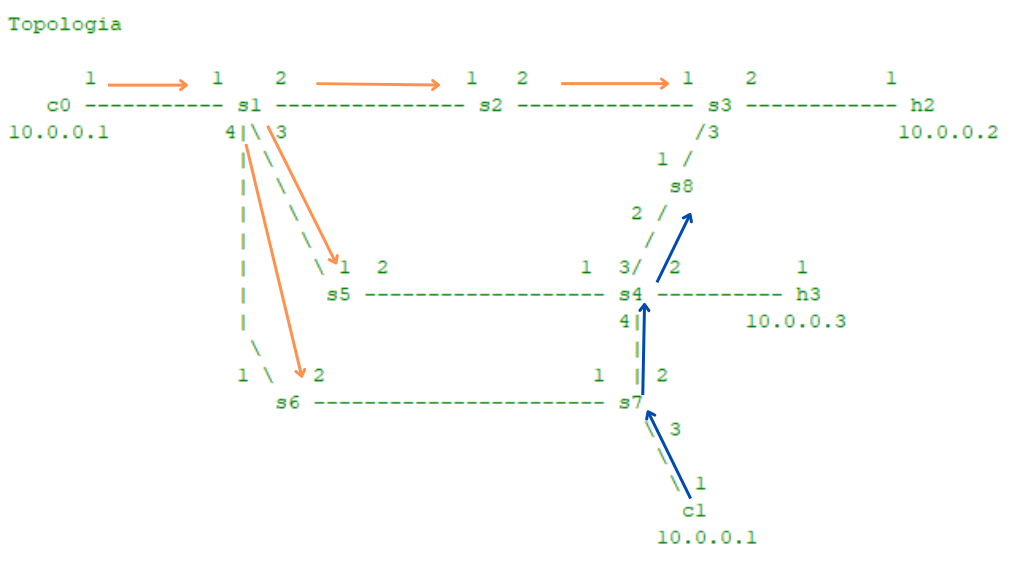
\includegraphics[width=\textwidth]{img/escenario1_2c_5}
 			\caption{Orden de conexión del experimento 6}
 		\end{minipage}
 		\hfill
 		\begin{minipage}[b]{0.35\textwidth}
 			\centering
 			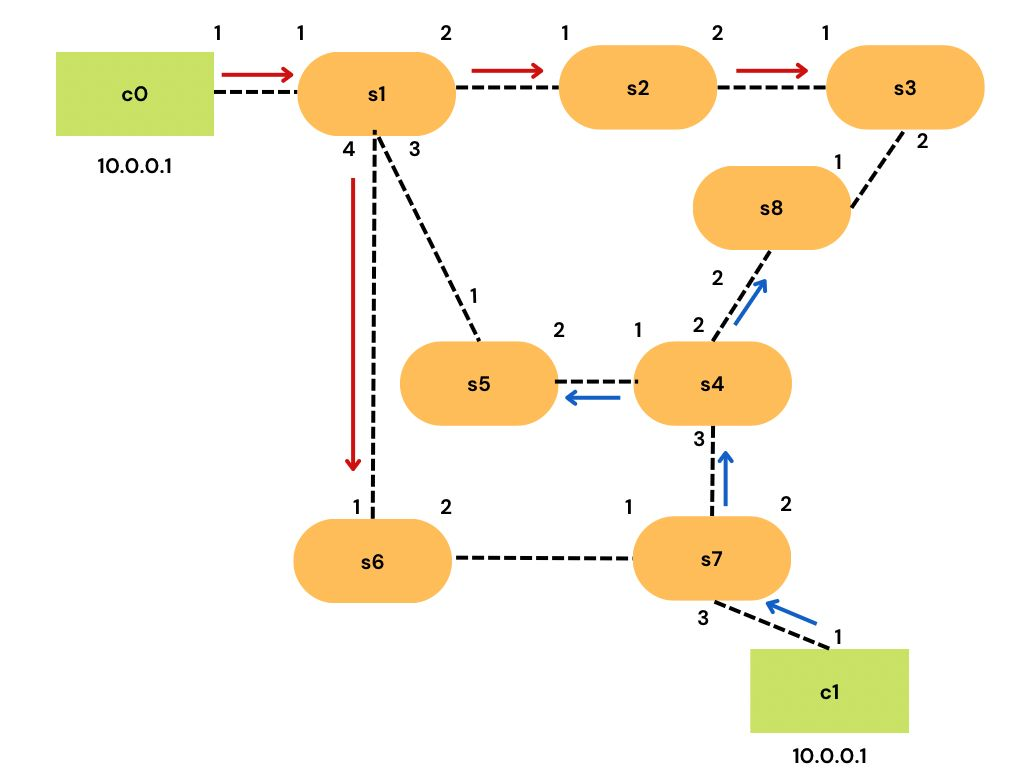
\includegraphics[width=\textwidth]{img/escenario1_2c_6}
 			\caption{Orden de conexión del experimento 7}
 		\end{minipage}
 		
 		\vspace{10pt} % Ajusta el espacio vertical entre las filas
 		
 		\begin{minipage}[b]{0.35\textwidth}
 			\centering
 			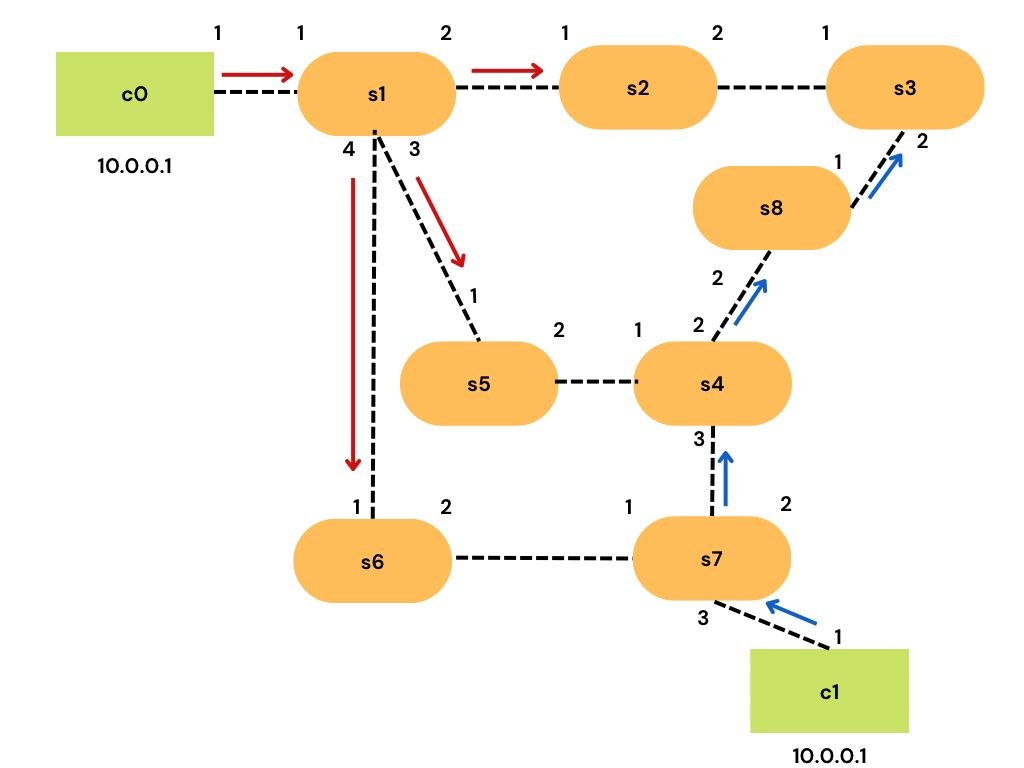
\includegraphics[width=\textwidth]{img/escenario1_2c_7}
 			\caption{Orden de conexión del experimento 8}
 		\end{minipage}
 		\hfill
 		\begin{minipage}[b]{0.35\textwidth}
 			\centering
 			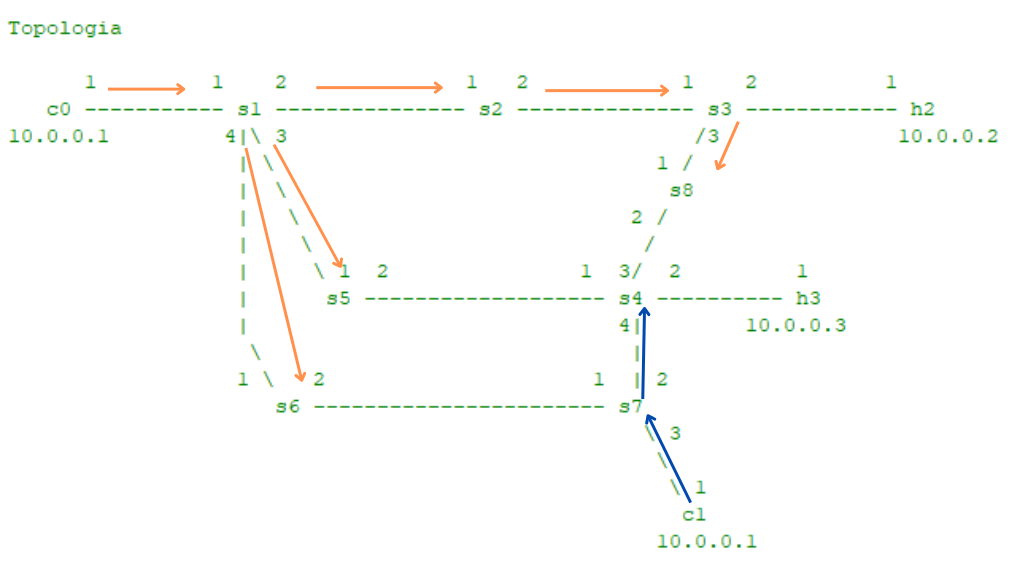
\includegraphics[width=\textwidth]{img/escenario1_2c_8}
 			\caption{Orden de conexión del experimento 10}
 			\label{figura:16}
 		\end{minipage}
 	\end{figure}
 	
	En estas figuras se muestra en color rojo el árbol de switches conectado al controlador c0 y en azul los switches conectados al controlador c1.
 	
 	Como podemos comprobar, pese a haber 10 experimentos, hemos podido ver 8 formas diferentes de conectar los switches. Estos resultados muestran la flexibilidad que tiene Periplus a la hora de realizar conexiones, que en escenarios más grandes dará lugar a repartos equilibrados entre los controladores.
 	
 	El reparto de switches por controlador es homogéneo en la mayor parte de las 10 ejecuciones. En la última ejecución, como se puede ver en la figura \ref{figura:switchesporcontrollerescenario1} el reparto se ha realizado de forma muy diferente: 6 switches se han conectado al controlador c0 y 2 switches al controlador c1. Esto se debe a que el controlador c1 ha arrancado después, con un pequeño retraso, dando el tiempo suficiente a que el controlador c0 haya ido avanzando con la gestión de switches. 
 	
 	\begin{figure}[H]
 		\centering
 		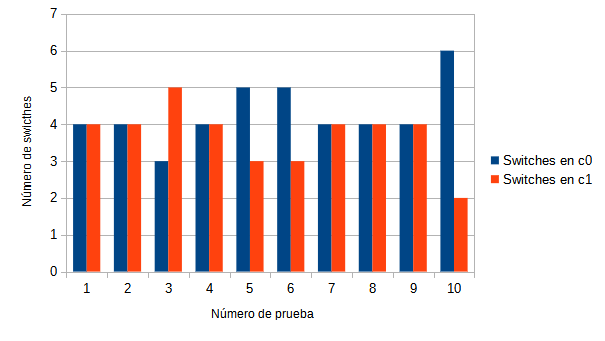
\includegraphics[width=16cm, keepaspectratio]{img/switchesporcontrollerescenario1}
 		\caption{Número de switches por controlador.}
 		\label{figura:switchesporcontrollerescenario1}
 	\end{figure}
 	
 	
 	
 	\clearpage
 	\section{Escenario 2}
 	
 	En la figura \ref{figura:escenario2-1c} se muestra un escenario más complejo formado por 16 switches y un único
 	controlador c0. La figura \ref{figura:escenario2-4c} muestra la misma topología con 4 controladores.
 		
 	En este escenario se espera una mejora muy superior en el tiempo de conexión de todos los switches al introducir varios controladores, ya que en el ejemplo con 1 controlador hay hasta 6 saltos hasta el switch más lejano, y con 4 controladores se reduce a 3, por lo que a priori podríamos esperar una mejora bastante superior a la obtenida en el primer escenario.
 	
 	\begin{figure}[H]
 		\centering
 		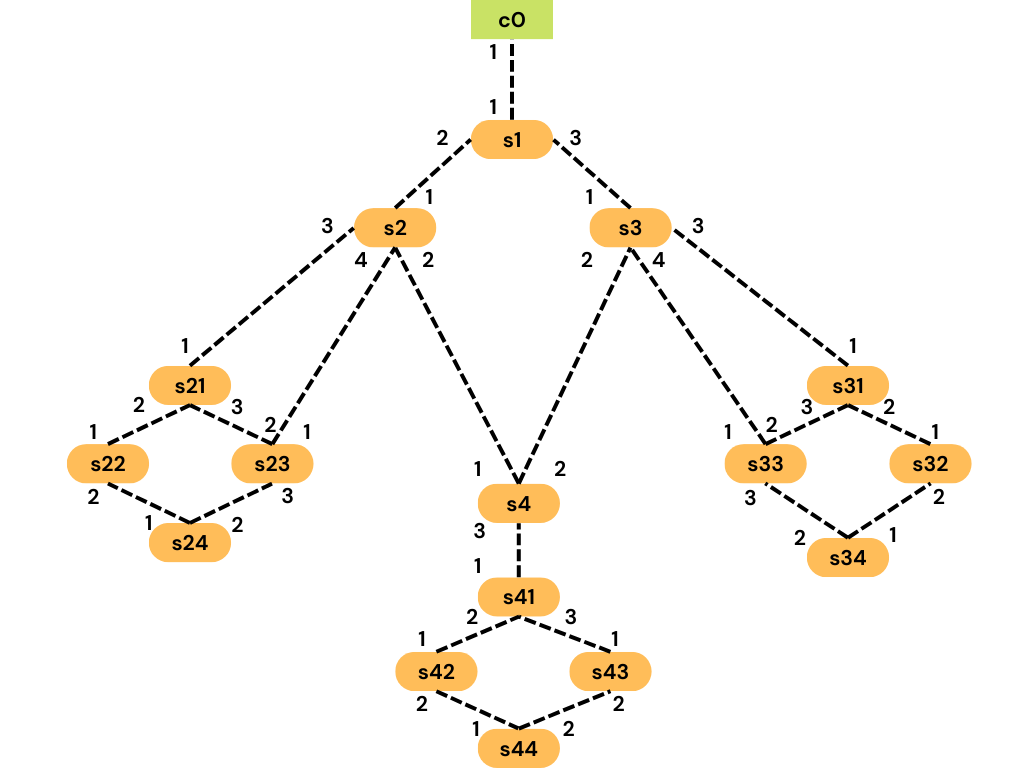
\includegraphics[width=16cm, keepaspectratio]{img/escenario2-1}
 		\caption{Segundo escenario con 1 controlador y 16 switches}
 		\label{figura:escenario2-1c}
 	\end{figure}
 	
 	\begin{figure}[H]
 		\centering
 		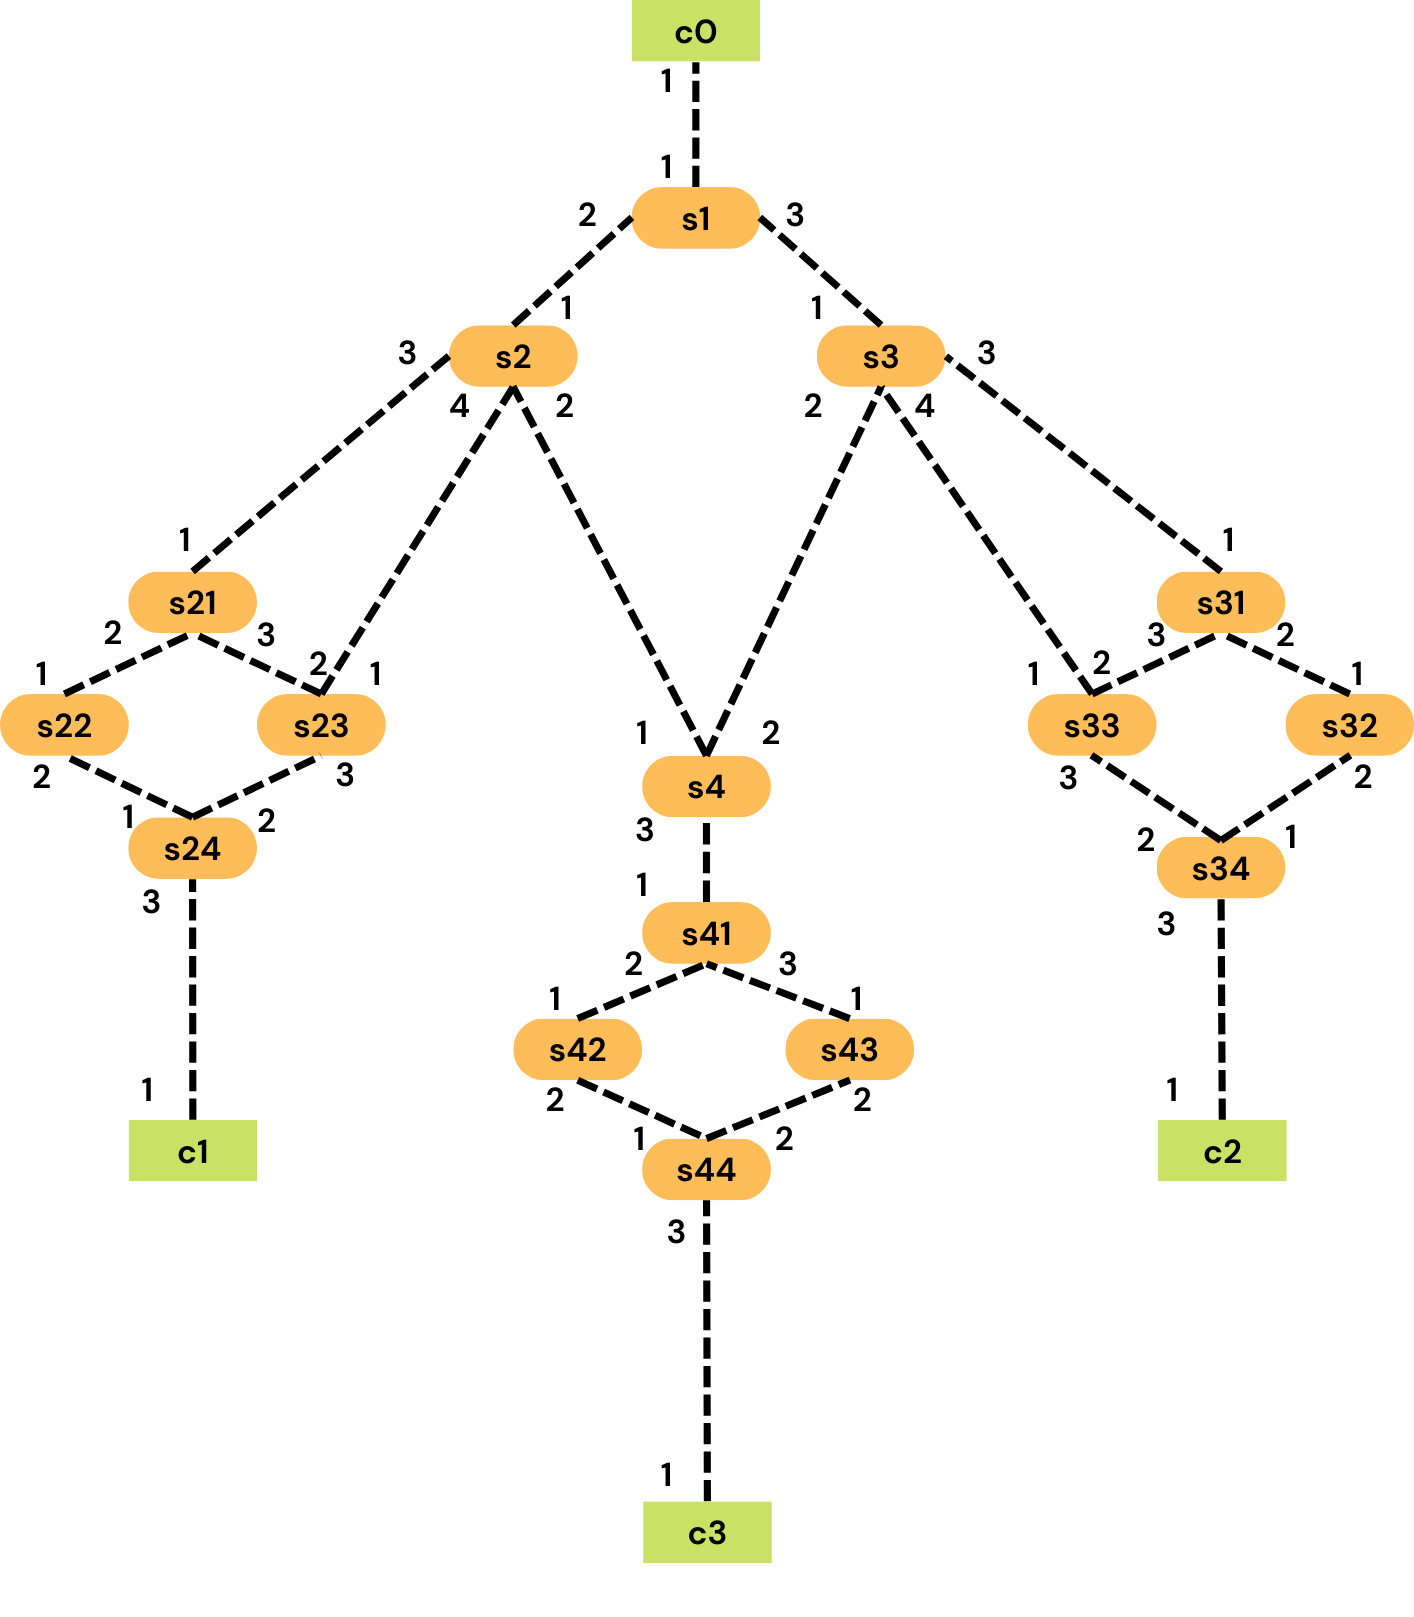
\includegraphics[width=14cm, keepaspectratio]{img/escenario2-2}
 		\caption{Segundo escenario con 4 controladores y 16 switches}
 		\label{figura:escenario2-4c}
 	\end{figure}
 	
 	Los resultados de las pruebas del tiempo de conexión de todos los switches se muestran en las figuras \ref{figura:comparativamesh} y \ref{figura:mediamesh}. A la vista de estos resultados podemos confirmar lo visto en el escenario 1 y lo que esperábamos antes de ver los resultados, ya que además en este escenario, al ser más grande y complejo, la disminución es mas notoria. El tiempo máximo de conexión en los switches se ha reducido en 0.1464 segundos, siendo el sistema un 26.28 \% mas rápido con 4 controladores que con 1.
 	
 	%Figura comparativa de tiempos en el segundo escenario
 	\begin{figure}[H]
 		\centering
 		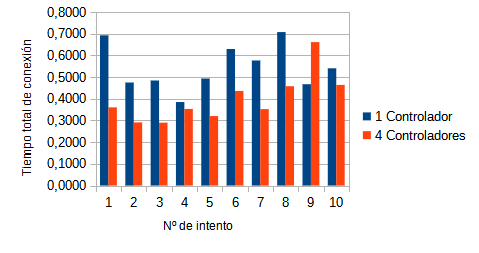
\includegraphics[width=16cm, keepaspectratio]{img/comparativamesh}
 		\caption{Tiempo que tardan todos los switches del escenario 2 en estar gestionados por un controlador.}
 		\label{figura:comparativamesh}
 	\end{figure}
 	
 	
 	%Figura comparativa de medias en el segundo escenario
 	\begin{figure}[H]
 		\centering
 		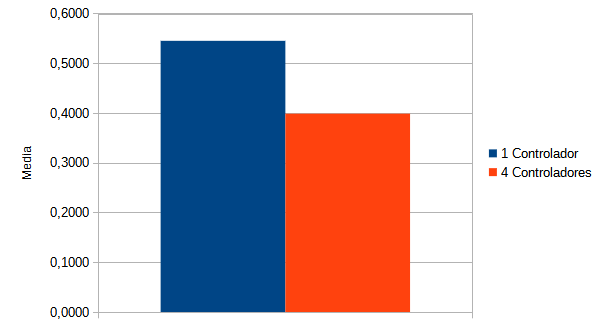
\includegraphics[width=12cm, keepaspectratio]{img/comparativamediamesh}
 		\caption{Comparativa de media de tiempos en conseguir que todos los switches del escenario 2 estén gestionados por un controlador.}
 		\label{figura:mediamesh}
 	\end{figure}
 	
 	
 	Y como puede verse en las figuras \ref{fig:medianamesh} y \ref{fig:varianzamesh}, también hay bastante diferencia en la mediana y la varianza. Al haber 4 controladores, es difícil que haya tiempos muy altos, de ahí que se reduzca la mediana y la varianza.
 	

\begin{figure}[H]
	\centering
	\begin{minipage}[b]{0.45\textwidth}
		\centering
		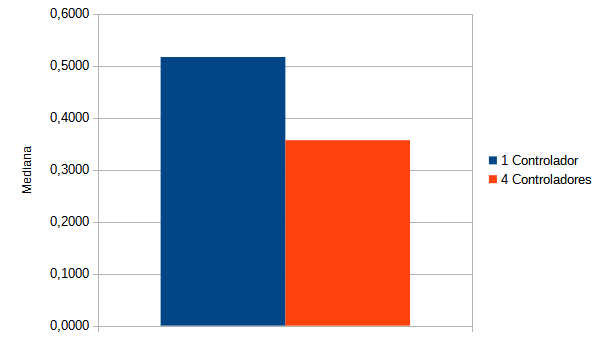
\includegraphics[width=\textwidth]{img/comparativamedianamesh}
		\caption{Comparativa de medianas en conseguir que todos los switches del escenario 2 estén gestionados por un controlador}
		\label{fig:medianamesh}
	\end{minipage}
	\hfill
	\begin{minipage}[b]{0.45\textwidth}
		\centering
		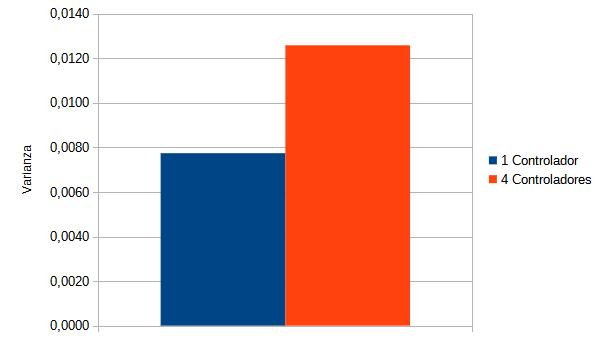
\includegraphics[width=\textwidth]{img/comparativavarianzamesh}
		\caption{Comparativa de varianza en conseguir que todos los switches del escenario 2 estén gestionados por un controlador}
		\label{fig:varianzamesh}
	\end{minipage}
\end{figure}
 	
 	\vspace{10pt} 
 	
 	Además, hemos comprobado que por lo general el reparto de switches entre los controladores se ha realizado de forma bastante equitativa como puede verse en la figura \ref{figura:switchesporcontrollermesh}. El reparto desigual de los últimos experimentos se asocia a un fallo de la máquina al realizar los experimentos, algo que ha ocurrido en los escenarios más grandes debido a la gran carga de trabajo que tenía el ordenador al realizar las simulaciones. 
 	
 	
 	\begin{figure}[H]
 		\centering
 		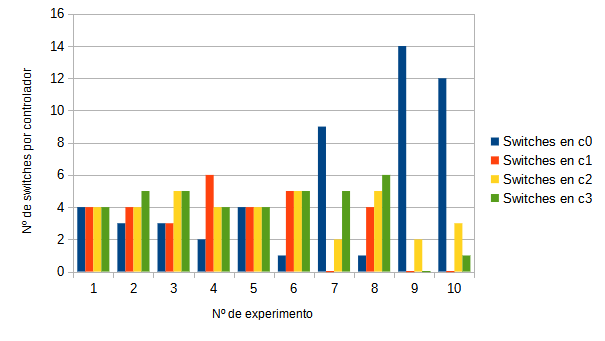
\includegraphics[width=16cm, keepaspectratio]{img/switchesporcontrollermesh}
 		\caption{Número de switches por controlador en el escenario 2}
 		\label{figura:switchesporcontrollermesh}
 	\end{figure}
 	
 	
 	\clearpage
 	\section{Escenario 3}
 	 
 	A continuación, se llevará a cabo un análisis de un escenario con mayor número de caminos alternativos (figura \ref{figura:b4_1}) y el mismo escenario con 2 controladores en vez de 1 (figura \ref{figura:b4_2}), para ver cómo reacciona Periplus en este caso.
 	En el escenario con un controlador, vemos que el switch mas lejano está a 4 saltos, mientras que el escenario con dos controladores el switch mas lejano está a 3 saltos. Lo curioso de este escenario es la gran cantidad de conexiones entre switches que hay, y que el segundo controlador se coloca en el extremo más lejano, pero lejos de otra gran parte de los switches.
 	
 	%Figura comparativa de tiempos en el tercer escenario
 	\begin{figure}[H]
 		\centering
 		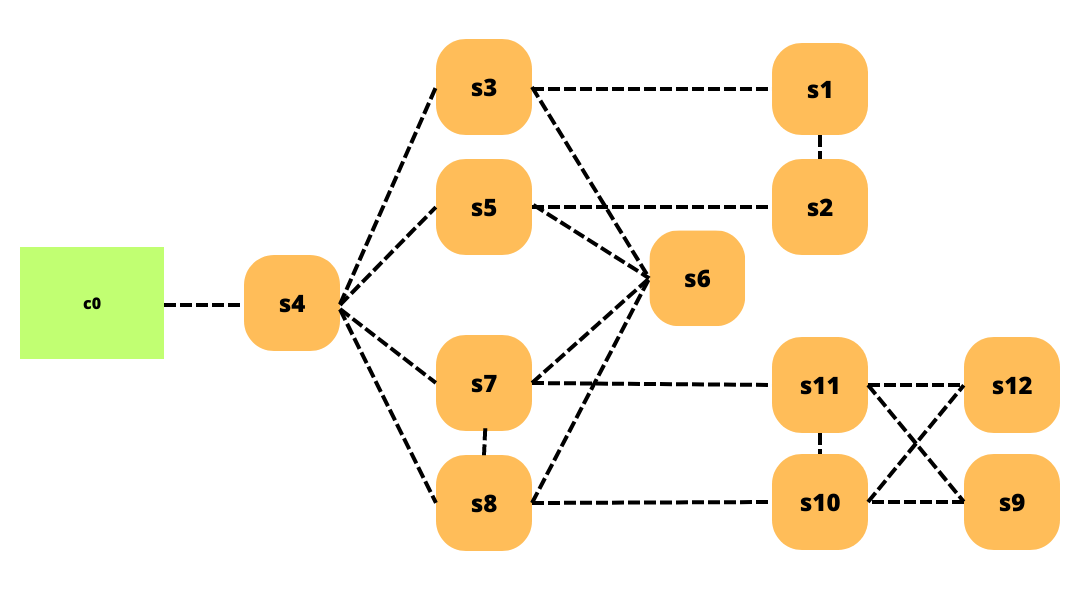
\includegraphics[width=14cm, keepaspectratio]{img/b4_1}
 		\caption{Tercer escenario con 1 controlador y 12 switches}
 		\label{figura:b4_1}
 	\end{figure}
 	
 	%Figura comparativa de medias en el tercer escenario
 	\begin{figure}[H]
 		\centering
 		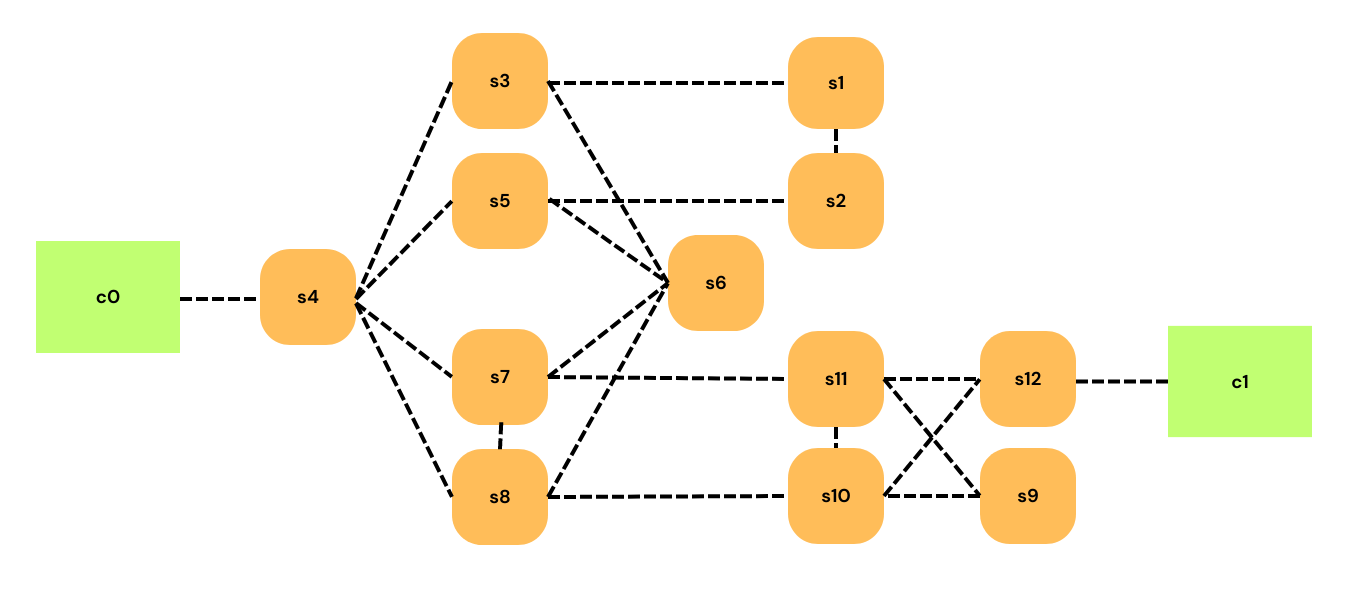
\includegraphics[width=14cm, keepaspectratio]{img/b4_2}
 		\caption{Tercer escenario con 2 controladores y 12 switches}
 		\label{figura:b4_2}
 	\end{figure}
 	
 	En las figuras \ref{figura:comparativab4} y figura \ref{figura:mediab4} se muestran los resultados obtenidos. Podemos confirmar lo visto en los anteriores escenarios. En este escenario, al ser más complejo en número de caminos alternativos, la disminución es más notoria. El tiempo máximo de conexión en los switches se ha reducido en 0.168 segundos, siendo el sistema un 47.19 \% más rápido con 2 controladores que con 1.
 	
	En este escenario se observa claramente que cuanto menor es el número de saltos entre el controlador y los switches, menor es el tiempo de conexión total de todos los switches.
 	
 	\begin{figure}[H]
 		\centering
 		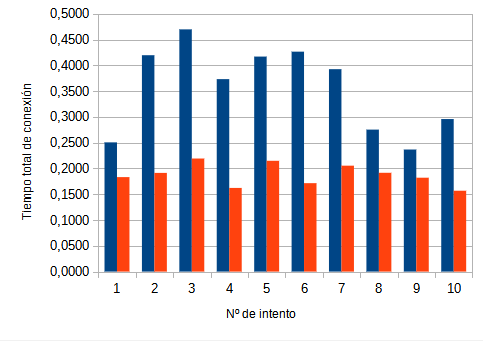
\includegraphics[width=12cm, keepaspectratio]{img/comparativaescenario3}
 		\caption{Comparativa de tiempos en el tercer escenario}
 		\label{figura:comparativab4}
 	\end{figure}
 	
 	
 	
 	\begin{figure}[H]
 		\centering
 		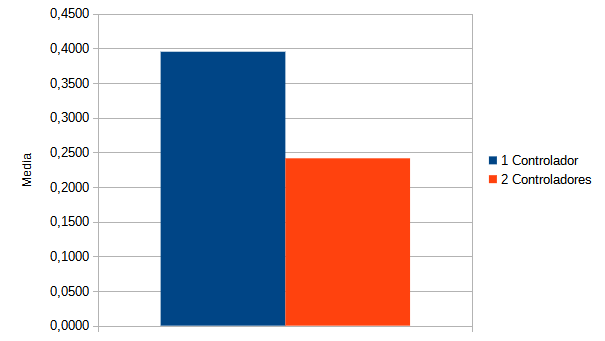
\includegraphics[width=12cm, keepaspectratio]{img/comparativamediaescenario3}
 		\caption{Comparativa de media de tiempos en el tercer escenario}
 		\label{figura:mediab4}
 	\end{figure}
 	
 	En las figuras \ref{fig:medianascenario3} y \ref{fig:varianzaescenario3} se observa también que hay bastante diferencia en la mediana y la varianza. Al haber 2 controladores y tantos caminos alternativos, es difícil que haya tiempos muy altos, de ahí que se reduzca la mediana y sobretodo la varianza.
 	
 	\begin{figure}[H]
	 	\centering
	 	\begin{minipage}[b]{0.45\textwidth}
	 		\centering
	 		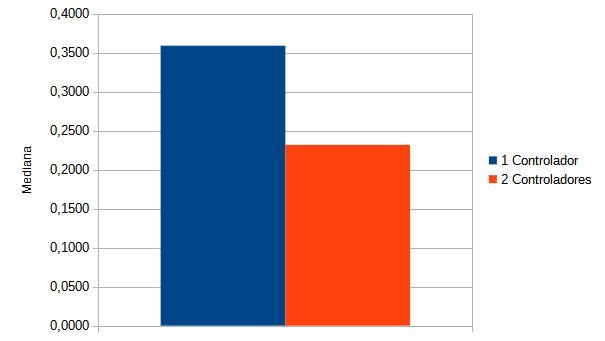
\includegraphics[width=\textwidth]{img/comparativamedianaescenario3}
	 		\caption{Comparativa de medianas en conseguir que todos los switches del escenario 3 estén gestionados por un controlador}
	 		\label{fig:medianascenario3}
	 	\end{minipage}
	 	\hfill
	 	\begin{minipage}[b]{0.45\textwidth}
	 		\centering
	 		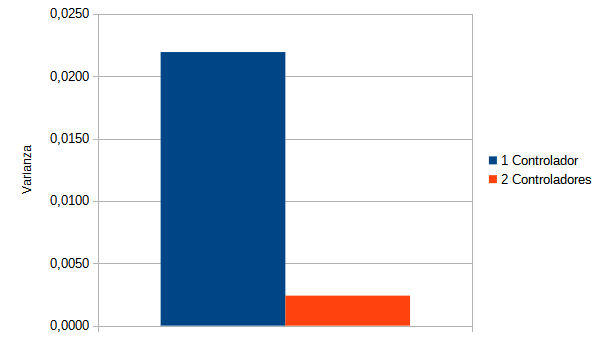
\includegraphics[width=\textwidth]{img/comparativavarianzaescenario3}
	 		\caption{Comparativa de varianza en conseguir que todos los switches del escenario 3 estén gestionados por un controlador}
	 		\label{fig:varianzaescenario3}
	 	\end{minipage}
 	\end{figure}
 	
 	En la figura \ref{figura:switchesporcontrollerb4} se observa que el reparto de switches entre los controladores se ha realizado de forma previsible. El primer controlador acapara más switches conectados en cada experimento, debido a que tiene una mayor cantidad de switches más cerca que el segundo controlador.
 	
 	
 	\begin{figure}[H]
 		\centering
 		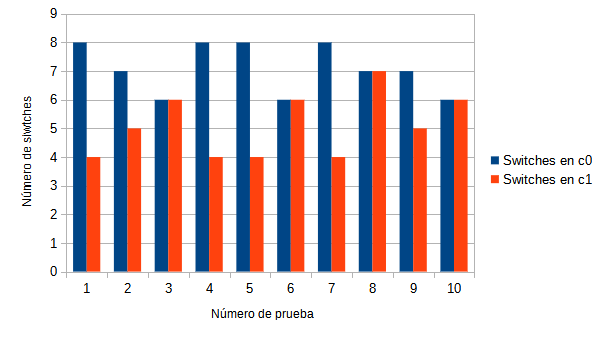
\includegraphics[width=14cm, keepaspectratio]{img/switchesporcontrollerescenario3}
 		\caption{Número de switches por controlador en el tercer escenario.}
 		\label{figura:switchesporcontrollerb4}
 	\end{figure}
 	
 	En este caso no se incluyen las figuras que muestran los switches conectados a cada controlador porque los resultados muestran que en cada ejecución se ha obtenido un árbol de conexión diferente debido a la existencia de varios caminos alternativos e igual distancia al controlador.
	
	\clearpage
	\section{Escenario 4}
	
	En este último experimento y a diferencia de los escenarios anteriores, se realizará una tercera comparación, ya que estudiaremos un escenario con uno, dos, y cuatro controladores, para comprobar cómo cambia en función de cada caso.
	En la figura \ref{figura:e4_1} podemos observar el primer caso, un único controlador para 20 switches, en la figura \ref{figura:e4_2} tenemos el mismo escenario pero con 2 controladores para los 20 switches y la figura \ref{figura:e4_3} tiene 4 controladores para los 20 switches.
	
	En este escenario, el número de saltos no va a disminuir, ya que se va a mantener la misma distancia máxima entre los controladores y los switches más alejados, pero se esperan tiempos más bajos debido a que el reparto de switches se debería dividir por 2 y 4 respectivamente.
	
	\begin{figure}[H]
		\centering
		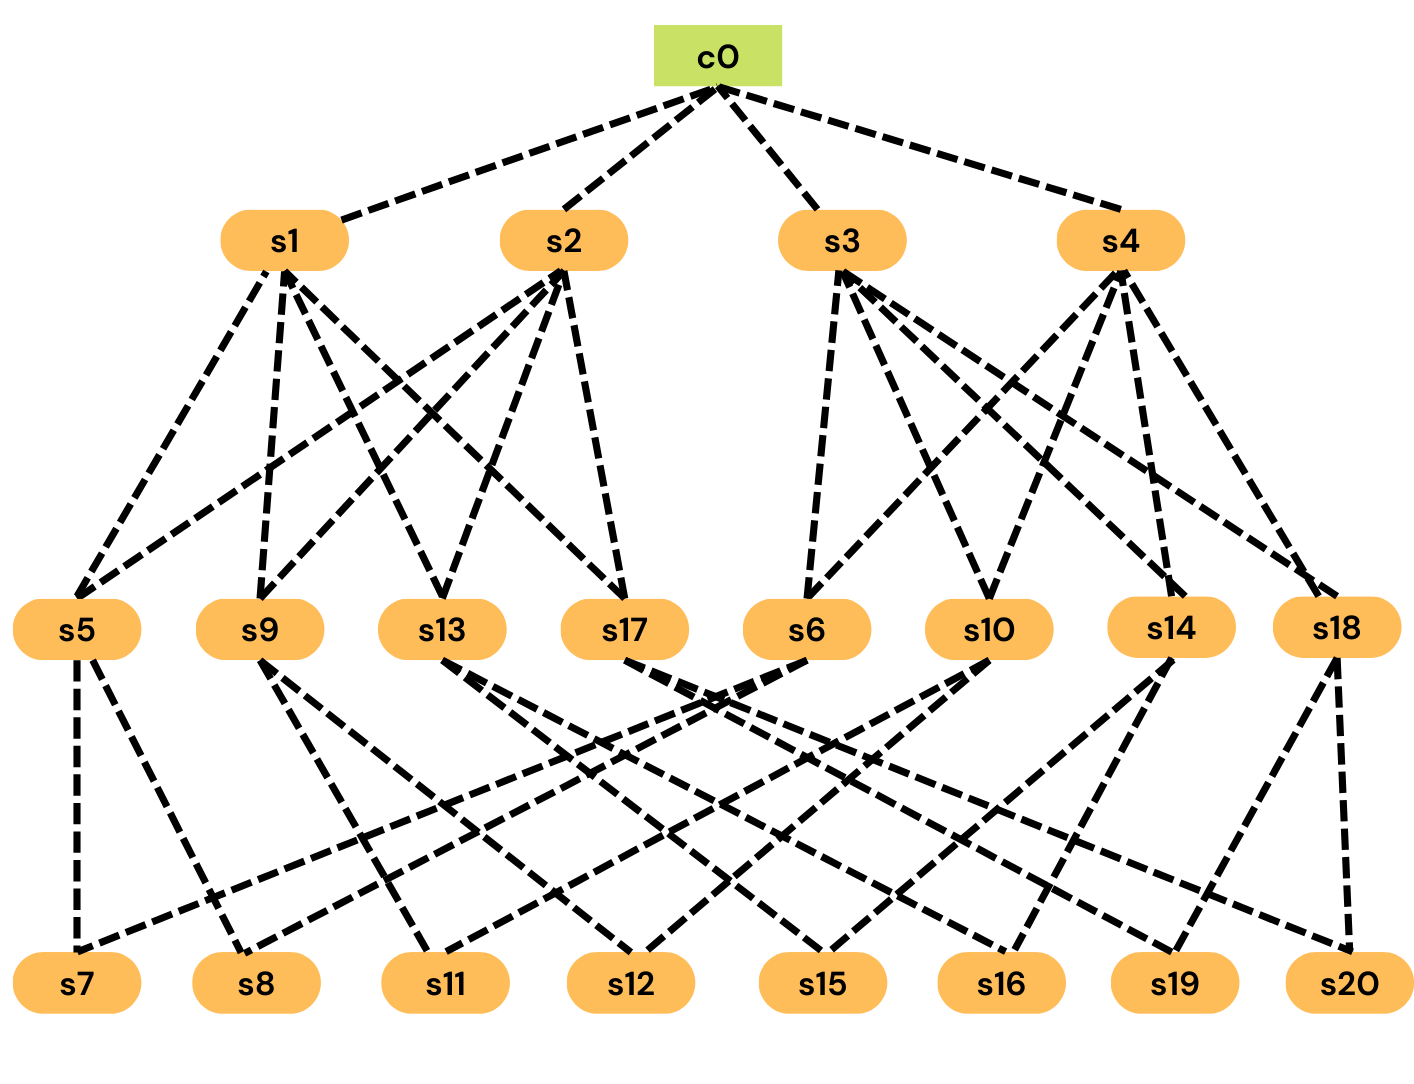
\includegraphics[width=16cm, keepaspectratio]{img/e4_1}
		\caption{Cuarto escenario con 1 controlador y 20 switches}
		\label{figura:e4_1}
	\end{figure}
	
	\begin{figure}[H]
		\centering
		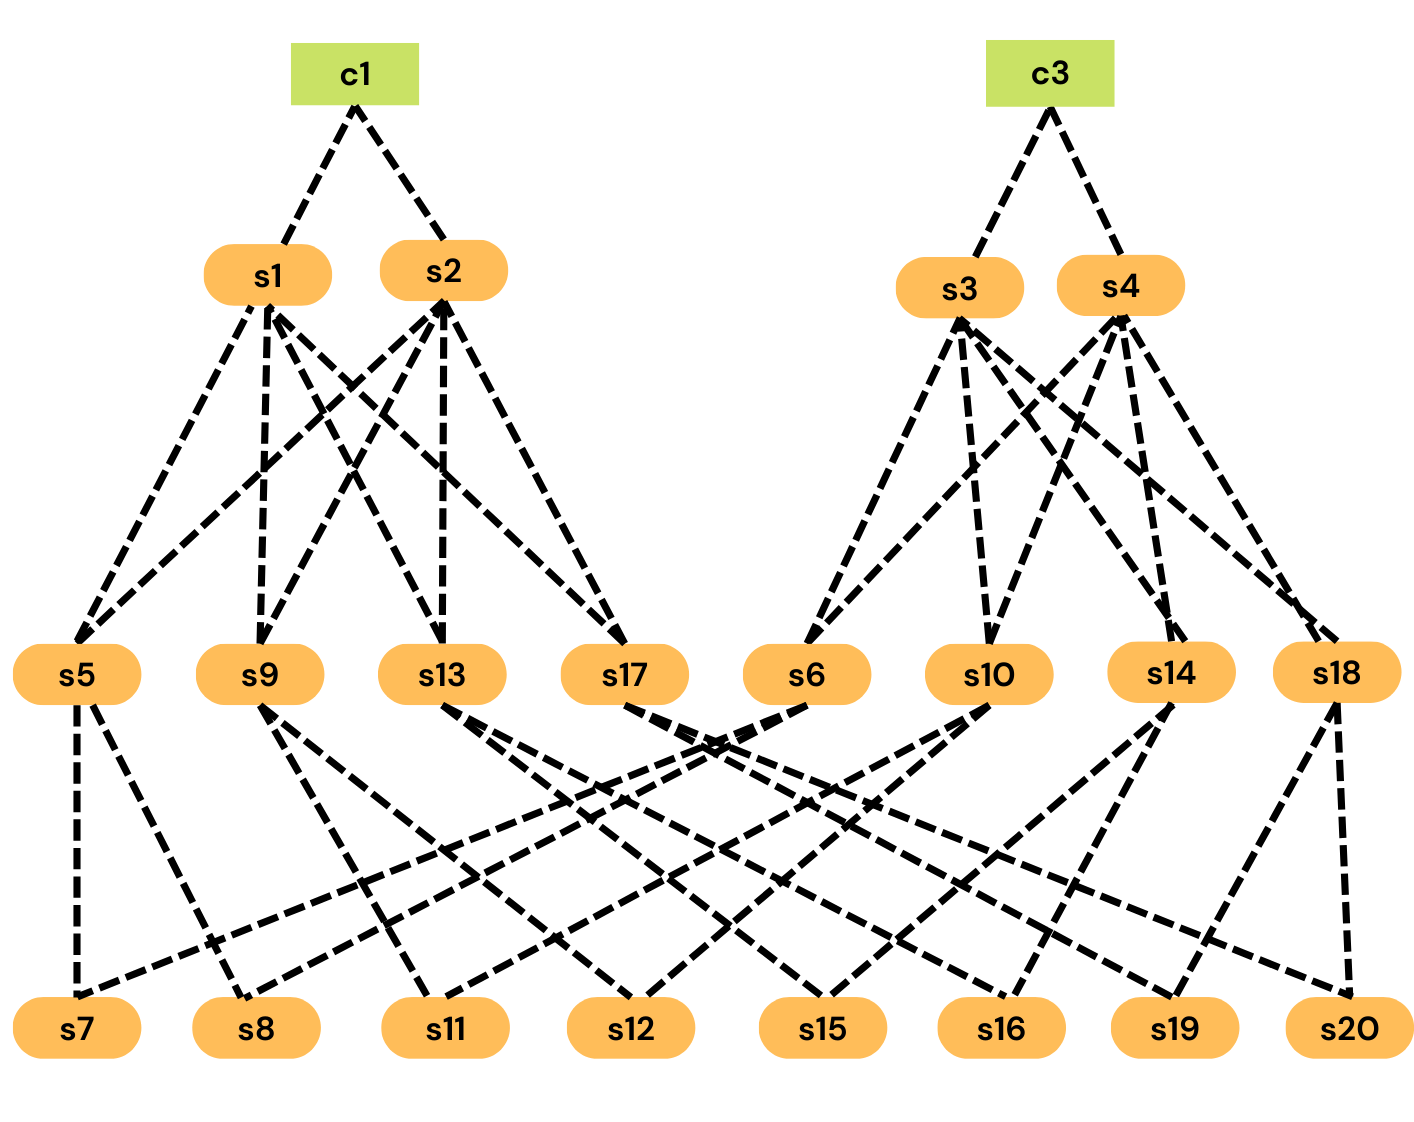
\includegraphics[width=13cm, keepaspectratio]{img/e4_2}
		\caption{Cuarto escenario con 2 controladores y 20 switches}
		\label{figura:e4_2}
	\end{figure}
	
	
	\begin{figure}[H]
		\centering
		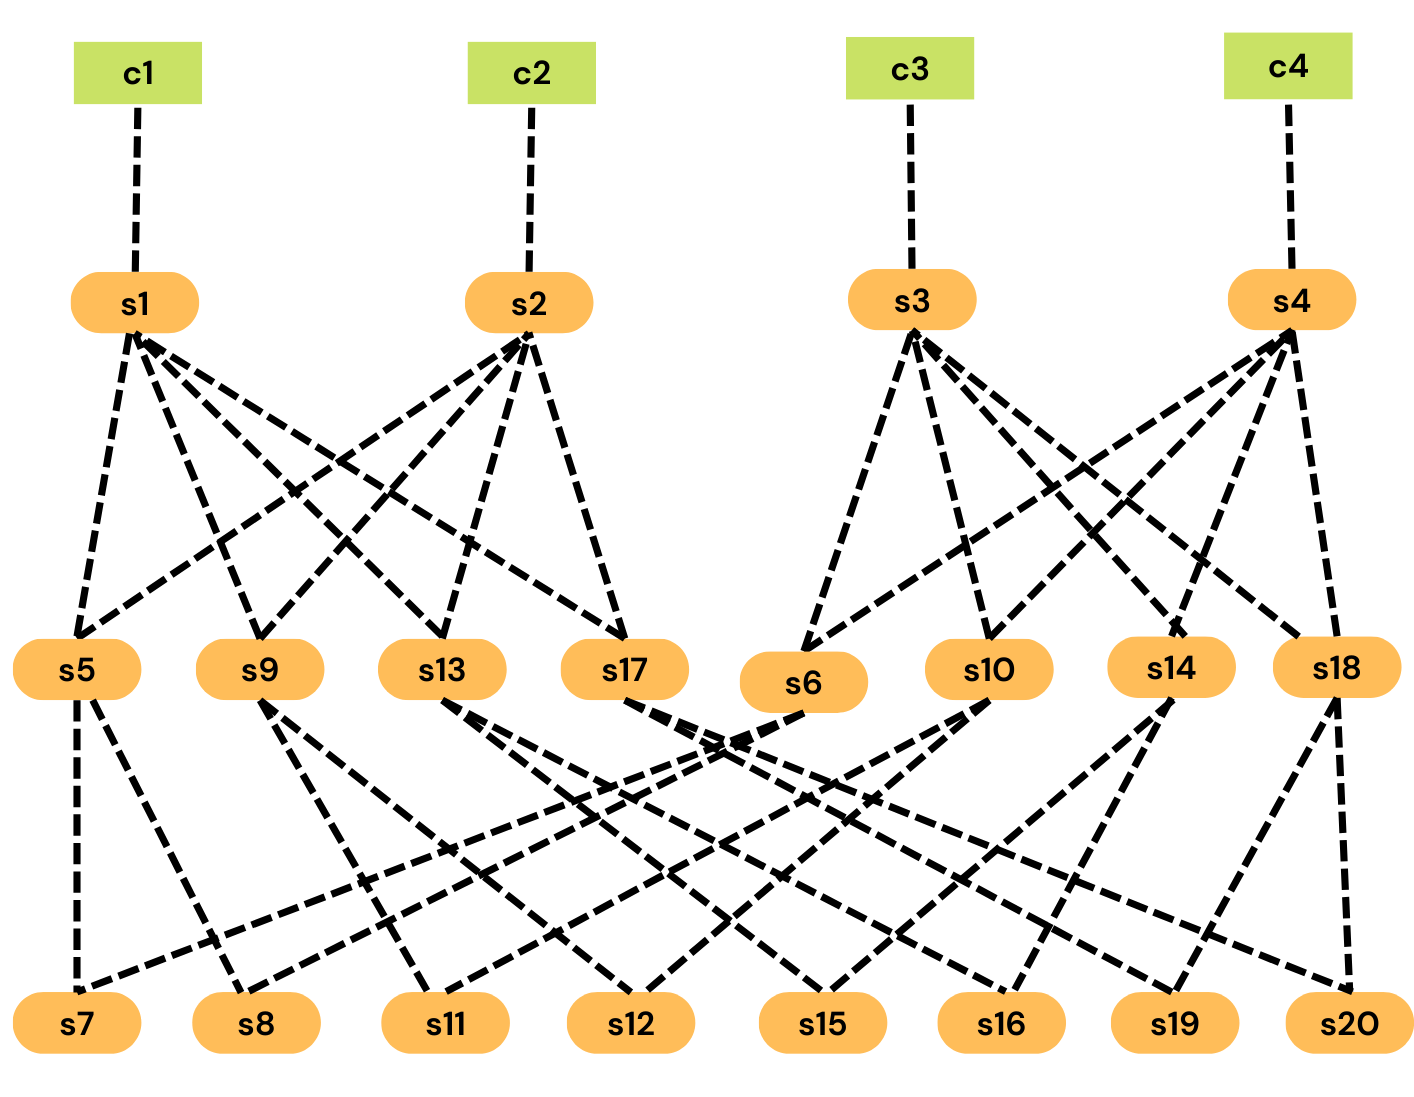
\includegraphics[width=13cm, keepaspectratio]{img/e4_3}
		\caption{Cuarto escenario con 4 controladores y 20 switches}
		\label{figura:e4_3}
	\end{figure}
	
En las figuras \ref{figura:comparativaescenario4} y \ref{figura:mediaescenario4} podemos observar la comparación del escenario con 1 y 2 controladores en tiempos y medias. Con estos resultados vemos que no solo influye el número de saltos entre el controlador y switch, sino que también es importante la carga de trabajo que va a tener cada controlador. El tiempo máximo de conexión de todos los switches se ha reducido en 0.168 segundos, siendo el sistema un 47.19 \% más rápido con 2 controladores que con 1. Teniendo en cuenta que la carga de trabajo se ha repartido entre 2, podemos observar que para escenarios complejos, cuantos más controladores haya, más rápida será la configuración de los switches, además del factor número de saltos al controlador desde el switch más lejano.
		
		
	
	
	\begin{figure}[H]
		\centering
		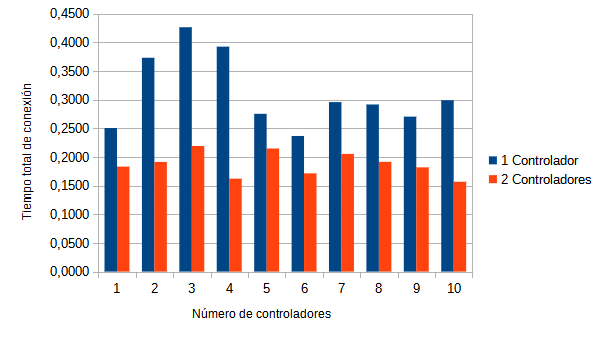
\includegraphics[width=12cm, keepaspectratio]{img/comparativaescenario4}
		\caption{Tiempo que tardan todos los switches del escenario 4 en estar gestionados por un controlador.}
		\label{figura:comparativaescenario4}
	\end{figure}
	
	\begin{figure}[H]
		\centering
		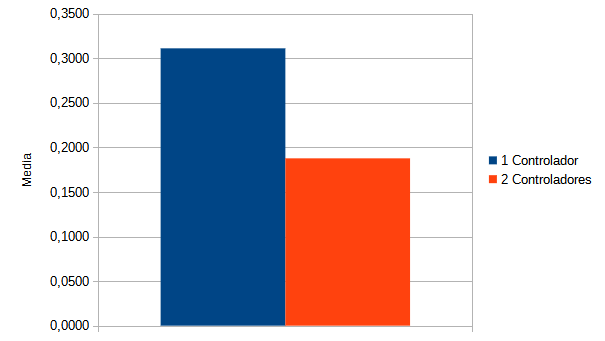
\includegraphics[width=10cm, keepaspectratio]{img/comparativamediaescenario4}
		\caption{Comparativa de media de tiempos en conseguir que todos los switches del escenario 4 estén gestionados por un controlador.}
		\label{figura:mediaescenario4}
	\end{figure}
	

	Como se puede observar en las figuras \ref{fig:medianascenario4} y \ref{fig:varianzaescenario4} también hay bastante diferencia en la mediana y la varianza. 
	
%	Además, hemos comprobado que por lo general el reparto de switches entre los controladores se ha realizado de forma correcta.
	\begin{figure}[H]
		\centering
		\begin{minipage}[b]{0.45\textwidth}
			\centering
			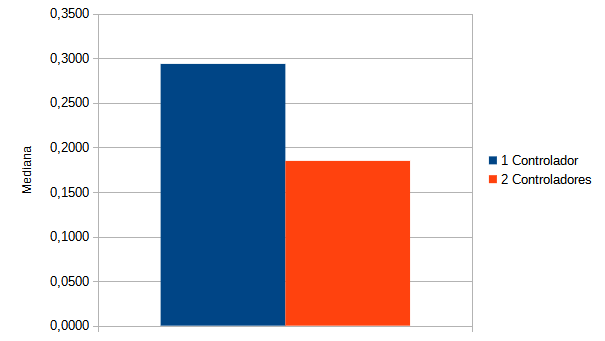
\includegraphics[width=\textwidth]{img/comparativamedianaescenario4}
			\caption{Comparativa de medianas en conseguir que todos los switches del escenario 4 estén gestionados por un controlador}
			\label{fig:medianascenario4}
		\end{minipage}
		\hfill
		\begin{minipage}[b]{0.45\textwidth}
			\centering
			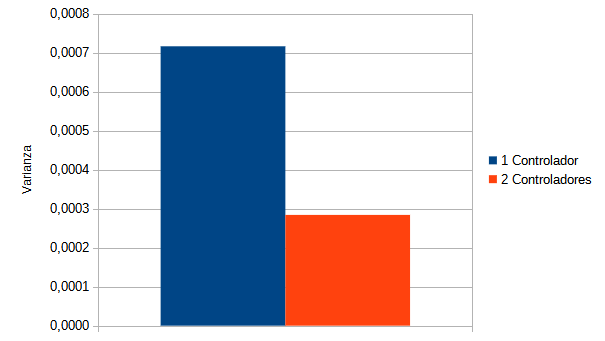
\includegraphics[width=\textwidth]{img/comparativavarianzaescenario4}
			\caption{Comparativa de varianza en conseguir que todos los switches del escenario 4 estén gestionados por un controlador}
			\label{fig:varianzaescenario4}
		\end{minipage}
	\end{figure}
	
		En la figura \ref{figura:switchesporcontrollerescenario4} se muestra que el reparto de switches entre los controladores se ha realizado de forma previsible. El primer controlador está conectado a más switches en cada experimento, debido a que en este escenario más complejo, el retraso que tiene el segundo controlador en arrancar da suficiente tiempo al primero para adelantarse en las conexiones.
		
	\begin{figure}[H]
		\centering
		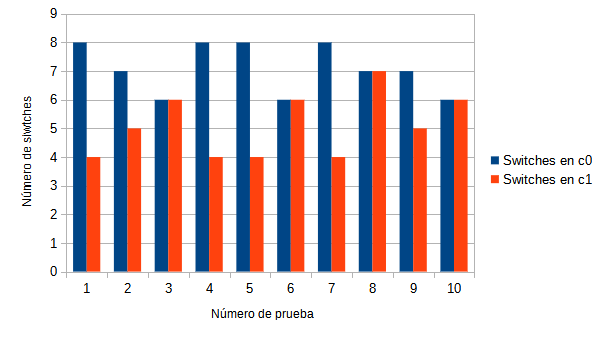
\includegraphics[width=14cm, keepaspectratio]{img/switchesporcontrollerescenario3}
		\caption{Número de switches por controlador en el escenario 4.}
		\label{figura:switchesporcontrollerescenario4}
	\end{figure}
	

	
En la figura \ref{figura:comparativaFail} podemos observar una comparativa del escenario con 1, 2 y 4 controladores.
	
	\begin{figure}[H]
		\centering
		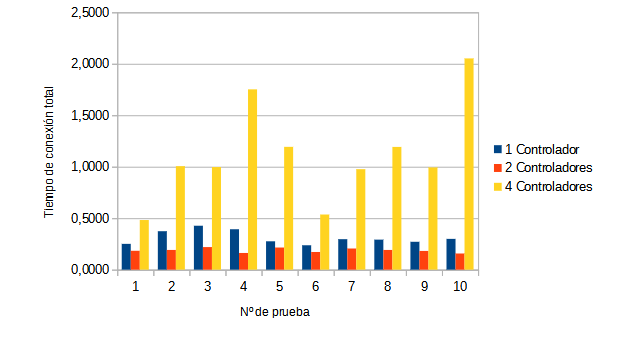
\includegraphics[width=16cm, keepaspectratio]{img/comparativaFail}
		\caption{Tiempo que tardan todos los switches del escenario 4 en estar gestionados por un controlador con 3 opciones diferentes.}
		\label{figura:comparativaFail}
	\end{figure}
	
	En la figura \ref{figura:comparativaFail} se observa que no ha habido mejora, sino que ha habido un empeoramiento muy  significativo. Puede ser debido a la sobrecarga de arrancar dentro de un escenario donde existen muchos caminos alternativos 4 controladores. En el arranque de un switch en este escenario podría ocurrir que el switch intentase la conexión simultánea con varios controladores provocando un retraso hasta que solo una de las conexiones con uno de los controladores se mantenga activa y se descarta el resto de intentos de conexión.
	
	
	%%%%%%%%%%%%%%%%%%%%%%%%%%%%%%%%%%%%%%%%%%%%%%%%%%%%%%%%%%%%%%%%%%%%%%%%%%%%%%%%
	%%%%%%%%%%%%%%%%%%%%%%%%%%%%%%%%%%%%%%%%%%%%%%%%%%%%%%%%%%%%%%%%%%%%%%%%%%%%%%%%
	% CONCLUSIONES %
	%%%%%%%%%%%%%%%%%%%%%%%%%%%%%%%%%%%%%%%%%%%%%%%%%%%%%%%%%%%%%%%%%%%%%%%%%%%%%%%%
	
	\clearpage
	\chapter{Conclusiones}
	\label{chap:conclusiones}
	
	Como conclusión de lo visto en los diferentes experimentos, podemos confirmar que añadir más de un controlador a un escenario va a ayudar, en la gran mayoría de los casos, a minimizar tiempos de conexión de todos los switches. Además, dicho tiempo mejorará cuanto más lejos estén los nuevos controladores entre ellos, ya que los controladores tendrán que dar menos saltos para llegar a los switches que se encontraban más lejanos, y por tanto, se reducirá el tiempo final.  Sería interesante poder hacer pruebas en una máquina con mayores recursos de CPU y memoria para poder mejorar los resultados del escenario 4.
	
	\section{Consecución de objetivos}
	\label{sec:consecucion-objetivos}
	
	Tal y como se explicó en el capítulo \ref{chap:objetivos}, se pretendía conocer mejor el funcionamiento de Periplus con respecto al número de controladores en diferentes escenarios. Se han realizado pruebas en las que hemos podido ver nuevas casuísticas que nos han ido aportando nueva información sobre el funcionamiento de Periplus. Con el primer escenario, que era el más pequeño y el que se puede estudiar más en profundidad, se han confirmado las hipótesis que planteamos. Al añadir nuevos controladores, en los switches más alejados con respecto al escenario de un único controlador, se redujo considerablemente el tiempo de conexión de todos los switches, además se obtuvo un reparto más equitativo de switches por controlador.
	
	Asimismo, con el último experimento, hemos comprobado que no siempre se obtiene ventajas al añadir controladores, ya que una sobrecarga de éstos puede empeorar significativamente nuestros resultados pese a acortar los caminos. También aporta más complejidad y puede provocar retardos inesperados debido a que los switches pueden estar simultáneamente conectándose a varios controladores.
	
	\section{Aplicación de lo aprendido}
	\label{sec:aplicacion}
	A lo largo del presente trabajo de fin de grado he podido aplicar conocimientos adquiridos en las siguientes asignaturas: 
	\begin{enumerate}
		\item Arquitectura de Redes de Ordenadores. Primer contacto con las redes de ordenadores, arquitectura TCP/IP, protocolos de comunicación, etc.
		\item Sistemas Telemáticos. Continuación de Arquitectura de Redes de Ordenadores, donde se profundizaba más en los protocolos de encamiento dentro de la arquitectura TCP/IP y en los algoritmos de control de congestión en TCP.
	\end{enumerate}
	
	
	\section{Lecciones aprendidas}
	\label{sec:lecciones_aprendidas}
	
	Para poder realizar el presente trabajo de fin de grado he tenido que adquirir conocimientos en lo que respecta a:
	
	\begin{enumerate}
		\item SDN y OpenFlow. Al ser la arquitectura de red utilizada en este trabajo. El protocolo OpenFlow establece la comunicación entre el controlador y los dispositivos de red mediante mensajes definidos. El controlador puede enviar instrucciones a los dispositivos de red, como reglas de enrutamiento o de flujo, y recibir información sobre el estado de la red, como estadísticas de tráfico. Esto permite una gestión centralizada y programable de la red, lo que facilita la implementación de políticas de red, la optimización del tráfico y la resolución de problemas.
		\item Controlador Periplus. Este controlador implementa un encaminamiento basado e origen que es un tipo de encaminamiento que no había estudiado previamente.
		\item LaTeX, ya que la memoria se ha realizado íntegramente con LaTeX. Con la ayuda de la plantilla publicada por el profesor Gregorio Robles y sus indicaciones, ha sido bastante sencillo realizar la documentación con dicha herramienta.
		\item Python. Pese a que el trabajo en sí no tenía programación, he tenido que aprender las bases del lenguaje para entender los scripts que se han utilizado tanto para definir los escenarios como para la realización de las pruebas.
		
	\end{enumerate}
	
	
	\section{Trabajos futuros}
	\label{sec:trabajos_futuros}
	
	Tras realizar el presente trabajo de fin de grado considero que sería una buena opción a tener en cuenta el optimizar los escenarios, creando lógica en los controladores, para que de forma coordinada puedan repartirse los switches, si tras el arranque el reparto hubiera quedado desequilibrado. Asimismo opino que podría ser interesante investigar sobre hasta qué punto es factible añadir controladores adicionales a un escenario, ya que posiblemente llegue un punto que la mejora no sea lo suficientemente satisfactoria. 
	Además, debido a lo ocurrido en el último experimento, creo que sería muy interesante formalizar los escenarios con diferente número de controladores, y ver cómo afectan estos controladores adicionales a la estabilidad del escenario y los tiempos de resolución de incidencias, con el objetivo de extraer una relación o ecuación para calcular el número óptimo de controladores por switches o por distancia, o por número de caminos alternativos a la misma distancia de un controlador o varios controladores.
	
	
	%%%%%%%%%%%%%%%%%%%%%%%%%%%%%%%%%%%%%%%%%%%%%%%%%%%%%%%%%%%%%%%%%%%%%%%%%%%%%%%%
	%%%%%%%%%%%%%%%%%%%%%%%%%%%%%%%%%%%%%%%%%%%%%%%%%%%%%%%%%%%%%%%%%%%%%%%%%%%%%%%%
	% APÉNDICE(S) %
	%%%%%%%%%%%%%%%%%%%%%%%%%%%%%%%%%%%%%%%%%%%%%%%%%%%%%%%%%%%%%%%%%%%%%%%%%%%%%%%%
	
	\cleardoublepage
	
	%%%%%%%%%%%%%%%%%%%%%%%%%%%%%%%%%%%%%%%%%%%%%%%%%%%%%%%%%%%%%%%%%%%%%%%%%%%%%%%%
	%%%%%%%%%%%%%%%%%%%%%%%%%%%%%%%%%%%%%%%%%%%%%%%%%%%%%%%%%%%%%%%%%%%%%%%%%%%%%%%%
	% BIBLIOGRAFIA %
	%%%%%%%%%%%%%%%%%%%%%%%%%%%%%%%%%%%%%%%%%%%%%%%%%%%%%%%%%%%%%%%%%%%%%%%%%%%%%%%%
	
	\cleardoublepage
	
	% Las siguientes dos instrucciones es todo lo que necesitas
	% para incluir las citas en la memoria
	\bibliographystyle{abbrv}
	\bibliography{memoria} 
	
	[1]  A robust and reactive
	OpenFlow In-Band SDN Control Plane
	Version 0.1. Autores Pedro de las Heras y Eva María Castro. 2022
	
	[2]  Página informativa de OpenFlow https://noviflow.com/the-basics-of-sdn-and-the-openflow-network-architecture/ 
		
	[3]  Guía de LaTex.  https://github.com/gregoriorobles/plantilla-memoria/blob/master/memoria.tex
	
	[4]  Foundations of Modern Networking: SDN, NFV, QoE, IoT, and Cloud By William Stallings 2015
	
	[5]  Introducción a namespaces https://man7.org/linux/man-pages/man8/ip-netns.8.html
	
	[6]  Introducción a openvswitch http://openvswitch.org
	
	[7]  Introducción a Mininet http://mininet.org
	
	[8]  Continuación Mininet https://www.youtube.com/live/90fBCO1MMTA?si=uVvZdvl4D7t8ntFw
	
	[9]  Documentación de Networking http://docs.openstack.org
	
	[10] Documentación Linux Networking https://www.opencloudblog.com/
	
	[11] Documentación Ryu https://ryu-sdn.org/
	
	[12] Documentación Wireshark https://www.wireshark.org/
	
	[13] Página oficial de OpenFlow https://opennetworking.org/wp-content/uploads/2013/04/openflow-spec-v1.0.0.pdf
	
 	
	 % memoria.bib es el nombre del fichero que contiene
	% las referencias bibliográficas. Abre ese fichero y mira el formato que tiene,
	% que se conoce como BibTeX. Hay muchos sitios que exportan referencias en
	% formato BibTeX. Prueba a buscar en http://scholar.google.com por referencias
	% y verás que lo puedes hacer de manera sencilla.
	% Más información: 
	% http://texblog.org/2014/04/22/using-google-scholar-to-download-bibtex-citations/
	
\end{document}
